\input{setup/preamble.tex}% package inclusion and set up of the document

\input{setup/macros.tex}% my new macros

\begin{document}
    %%% Prereport %%%
    \setlength\cftaftertoctitleskip{2pt}
    \setlength\cftafterloftitleskip{6pt}
    \setlength\cftafterlottitleskip{6pt}
    \selectlanguage{english}
    \title{Vessel}
    
    %%% Frontmatter Settings %%%
    \pagestyle{empty} %disable headers and footers
    \pagenumbering{roman} %use roman page numbering in the frontmatter I II...
    \fancyfoot[RE,LO]{17gr832} %page number on all pages
    \fancyfoot[LE,RO]{\thepage}
    \fancyhead[LE,LO,RE,RO]{}
    
    %%% Introductory Formalities %%%
    %\includepdf[pages={1}]{formalities/frontpage.pdf}
    \include{chapters/frontpage}
    \pagestyle{fancy}
    {\small
\strut\vfill % push the content to the bottom of the page
\noindent Aalborg University 2017 
\clearpage
    \input{formalities/titleSheet.tex}
    %%% Preface %%%
    %\cleardoublepage
    \chapter*{Preface}
\vspace{-12 pt}
The focus of this project is to design a control system for an autonomous surface vessel, such that it can navigate autonomously through a predetermined surface in the water.

This report has been written by a group of students on the second semester of the Master in Control and Automation at Aalborg University in the spring semester of 2017. It has been supervised by Jesper Abildgaard Larsen, associate professor at the Institute of Electronic Systems at Aalborg University.

The reader is expected to have a basic knowledge within physics and mathematics, as well as in modeling and linear control theory.

\textbf{Reading Instructions}
\vspace{-10 pt}
\begin{itemize}
    \item[-] The report is divided in three parts. Part I deals with the analysis of the system, which includes a description of the setup and the derivation of the dynamic model. Part II includes the control design, which contains the two approaches for an inner controller, the outer controller and the sensor fusion. Part III includes the results of the project, the discussion and the conclusion.
    \item[-] The report also includes appendixes that contain the journals for the different tests and other relevant information.
    \item[-] The bibliography is written using ISO 690, noted as [x], and it is included at the end of the report, after the appendixes.
    \item[-] An attachment is included as part of the report, and contains MATLAB scripts and simulations files, ROS files... \fxnote{Write what more is in the attachement}
\fxnote{Write reading instructions}
\end{itemize}

%
\textbf{Text by:}\\
\vspace{-12 pt}
\begin{table}[H]
	\centering
		\begin{tabular}{c c c}
			\underline{\phantom{JAERJAERJAERJAERGO}} & \phantom{cookies} & \underline{\phantom{JAERJAERJAERJAERGO}} \\
			Alejandro Alonso García & \phantom{cookies} & Anders Egelund Kjeldal \\
			&&\\
			\underline{\phantom{JAERJAERJAERJAERGO}} & \phantom{cookies} & \underline{\phantom{JAERJAERJAERJAERGO}} \\
			Himal Kooverjee & \phantom{cookies} & Niels Skov Vestergaard		\\
			&&\\
	    \multicolumn{3}{c}{\underline{\phantom{JAERJAERJAERJAERGO}}}\\
	    \multicolumn{3}{c}{Noelia Villarmarzo Arruñada}\\				
		\end{tabular}
\end{table}
\pagebreak
    
    \pdfbookmark[0]{Table of Contents}{label: tableOfContents}
    \tableofcontents
    \cleardoublepage
    
    %%% Mainmatter Settings %%%
    \pagenumbering{arabic} %use arabic page numbering in the mainmatter
    \fancyfoot[RO,LE]{\thepage \text{ of} \pageref{LastPage}}
    \fancyfoot[RE,LO]{17gr832}
    \fancyhead[RE,LO]{}
    \fancyhead[RE,LO]{\color{aaublue}\small\nouppercase\leftmark} %even page - chapter title
    \pagestyle{fancy}
    
    
    %%% PART 1 %%%
    \part{Pre-Analysis}
    
    %---------- Chapter 1 ---------------------------------------- Introduction
    \chapter{Introduction}

Brainstorm:

Autonomous surface vessels (ASV), applications\fxnote{sources needed on all this}:\\
- as a survey vessel performing measurements like bathymetry, temperature, flow in streams, Ph, NO2, NO3, ammonia, salt balance, etc.\\
- groundwater inflow in streams by analyzing temperature maps\\
- from all these measurements (and possibly more) it is possible to focus attention on problem areas both in biology and guidance of marine vessels.\\
- one strength of an ASV is that it can map out an entire stream, whereas manual measurements typicaly will be cumbersome and low in mapping resolution due to accessibility of the stream and time constraints/cost.\\
- for marine survey it can be useful as it can enter narrower and more shallow waters than larger manned vessels would be able to.\\
- the military has also been using ASV's for surveillance.

In this project the focus is first and foremost the control design, which will be realized with focus on bathymetric measurements. This will constitute a basis for setting up requirements for precision which will determine important parameters in the control design.

Why are bathymetric measurements generally interesting?\\
- used for efficient and safe guidance of marine vessels \fxnote{http://oceanservice.noaa.gov/facts/bathyuses.html}\\
- used in biological oceanography, as a for instance it can help in deciding which areas to protect for preservation of sea life \fxnote{http://oceanservice.noaa.gov/facts/bathyuses.html}\\
- is also a parameter used when analyzing streams \fxnote{more concrete source needed if this is to be included. The found source was no good, therefore it is not here.}

Specific case-study:
\fxnote{it could be very helpful if at all possible, since this would give concrete constraints for the precision that should be required of the control design.}
    
    %---------- Chapter 2 ---------------------------------------- Problem Analysis
    \chapter{Problem Analysis}
%
The goal of this project is to develop a control strategy that can make an autonomous surface vessel suitable for survey tasks in water. More specifically, it should be able to perform bathymetric measurements.

In order to set up the requirements for the control system it is helpful to study a more concrete case in which bathymetric measurements are already in use and where improvements in measurement techniques are desired.

The Port of Aalborg provides such a case along with previously used bathymetric measurements, see \autoref{fig:bathymetricMapPortOfAalborg}. These measurements are used by the Port of Aalborg to guide ships safely through the port without grounding.

\begin{figure}[H]
  \includegraphics[width=0.5\textwidth]{figures/smallDebthMapAalborg}
  \caption{A cut from the full bathymetric map found in \autoref{app:bathymetricMapPortOfAalborg} provided by the Port of Aalborg \fxnote{cite port of aalborg}.}
  \label{fig:bathymetricMapPortOfAalborg}
\end{figure}

The depths of the port are in constant change due to shifting sands on the bottom. So while the bathymetric measurements helps in guiding the ships by the safest route they are not currently provided frequently enough that this can be done in the most optimal manner. If two ships are headed towards each other, one of them will be forced to wait in places where there is sure to be enough space for both in order to allow them to pass each other. This however is sometimes an unnecessary precaution, had there been more recent knowledge of the depths in the port.\fxnote{who do we source for this?}

The measurements are currently performed from a manned vessel on which a multi beam echo sounder is installed. Contrary to single beam echo sounders, the multi beam can sweep a wider area. It is still however a time consuming task.\fxnote{more specifically how often, one or more boats, what exact kind of multi beam echo sounder is used?}

It is therefore desired to automate the process, preferably with a smaller unmanned vessel. This will allow for more frequent bathymetric measurements and the efficiency of guiding ships through the Port of Aalborg can be improved.

The vessel must be able to preform bathymetric measurements within an area autonomously. 
To do so it must be able to plan and follow a route, such that the entire area is measured. 
The route will be dependent on the sweep width of the sensor and the precision of the controller.
In order to ensure the entire area is covered, the path planner should include some overlap of the scanned areas, as this would account for potential inaccuracies of the system.


%The controller design must be able to track references provided by a path planer as well as rejecting disturbances such as possible wind or the effect of the waves. This requires a model of the disturbances to be included in the controller design along with a robust controller capable of handling model uncertainties.

%The path planer must be able to design a route, in the form of waypoints\fxnote{not necessarily, is it not too early to decide?}, to reach all the positions needed to perform the different measurements required for the survey.

%The accuracy and precision with which the route can be tracked has a significant impact on the efficiency of the system. The less closely the path is tracked, the more overlap of the echo sounder beam is required from each sweep in order to cover the entirety of the bottom.

The quality of the bathymetric measurements play part in determining the required overlap. Additionally other applications for the ASV would have requirements for the precision and accuracy provided by the control design. For these reasons and in order not to constrain the design to only one potential use, it is decided to set up some rather tight requirements for the system.

%%%%%Precision%%%%%%%%%%%
Following the S-44 IHO standards for hydrographic mapping, the measurements fall into the special category, which sets a maximum allowable horizontal uncertainty (THU) of 2 m, 95\% confidence level for the positional measurements. 
This standard is intended for under-keel measurements of the sea floor, which aligns with the scope of this project.\cite{IHO-S-44} 
The Canadian Hydrography Service (CHS) includes a stricter category, the Exclusive order. 
This category extends the special category to be more focused on shallow waters, such as harbors. 
This category sets the maximum THU to be 30 cm with a 95\% confidence interval. 
It have been decided to use this standard as this is the one that best resembles the intended use case of the system.\cite{CHS}
%From the project proposal it appears that a positioning accuracy of 0.1 m is desired. 
%From initial meetings with project supervisor, Jesper Abilgaard Larsen it was stated that a minimum precision of 0.3 m is required for the bathymetric measurements to be usable.\fxnote{Working on how to source this maybe use minutes?}

\section{Design Considerations}\label{sec:designconsiderations}
The system design assumes that the sensor used to measure the bottom of the fjord is based on the current multibeam echosounder used by the Port of Aalborg, the multibeam echosounder SeaBat 7125 \cite{echoSounder}, which has a swath angle of 140$^\mathrm{o}$.

Based on the bathymetric map found in \autoref{app:bathymetricMapPortOfAalborg}, a minimum depth can be considered to estimate the width of the beam when it reaches the bottom. This width is used to plan the trajectory that the boat needs to follow to be able to reach all the points in a given area, see \autoref{chap:outerController}. In \autoref{fig:echosounder} a diagram of the echosounder's beam can be seen.

\begin{figure}[H]
    \includegraphics[width=0.9\textwidth]{figures/echosounder}
    \caption{Diagram of the echosounder's beam.}
    \label{fig:echosounder}
\end{figure}

%%%%%Communication%%%%%%%%%%%
As the ASV is to be operated on water, it will be hard to access it during operation. 
As it is desired for to have access to the vessel at all times, some form of communication between a operator and the vessel must be established. 
This is crucial for the implementation of safety features such as emergency stops, redirecting the vessel or steer it back to land in case of system failures.

\section{Control Analysis}
For the vessel to autonomously survey an area, a controller is needed. 
The performance of the controller is crucial for how well the system preforms overall. 
One of the challenges when designing a controller is how well it handles disturbances. 
In the case of the vessel the disturbances are mostly represented as wind and wave disturbances. \fxnote{Should we mention the current}
\begin{figure}[H]
    \includegraphics[width=0.5\textwidth]{figures/boatdisturbance}
    \caption{Illustration of how the vessel is affected by disturbances.}
    \label{fig:boatdist}
\end{figure}

As illustrated on \autoref{fig:boatdist}, these external forces would alter the force vector of the vessel, influencing it's trajectory. 
If the controller is not sufficiently robust against this kind of noise, the vessel might not be able to follow a path, or do so with less precision, which then would needed to be compensated for. 
This would result in a loss in operating range, as the vessel would have to overlap a larger area to make sure the path covers the entirety of the survey area.

Additionally the controller could experience disturbances in regards to model inaccuracies. 
It is not possible to model a system perfectly, and will always be an approximation. 
These model variations influence the controllers performance as its design is based upon these. 

Another aspect of controller design is the energy consumption. 
The controller could be optimized such that it spends as little energy as possible reaching it's destination, giving the vessel a larger possible survey area. 

As the controller should be operational in most weather conditions, the robustness of the controller is considered the most important parameter. 



\section{Functional Requirements} \label{sec:requirements}
To be able to design a working prototype some functional requirements must be set and verified at the end of the project once all the design has been carried out.
%
\begin{enumerate}
  \item It should be possible to select the area in which the bathymetric measurements are to be performed.
  %\item A path planning algorithm should be able to plan a path within the selected area such that the bathymetric measurements can be performed.
  %\item The ASV should be able to track the path laid out by the path planning algorithm.
  \item The ASV should be able to autonomously plan and follow a route, such that the entire survey area is mapped.
  \item The controller should be robust to external disturbances.
  \item The ASV should record and store data locally for extraction at the end of the survey.
  \item It should be possible to give the ASV a command to stop and steer it back to land.
  \item THU not exceed 30cm with a 95\% confidence interval.
\end{enumerate}
%
%The remainder of the problem analysis will go into how the functional requirements can be achieved. This will result in a set of technical requirements, which sets the perimeters of the design.






%\section{Technical Requirements}
%\fxnote{this section should be placed after analysis of sensors}
%Track position reference:\\
%- Summary of results of sensor capabilities\\
%- precision requirements for the control design\\
%- The bathymetry measurements are reliant on how much the boat tips, as it is single beam and measures shortest distance in the beam, some analysis must be done in this regard. Maybe it is necessary to stabilize the boat with floats on its sides. It would still be sensitive to waves, maybe the problem can be solved by measuring the tilt of the boat and mapping the measurements to the correct point in the inertial system having used beam and tilt angle to calculate vertical distance. This approach will put the measurements in a band around the path of the boat rather than in a straight line, question is if this is a good or a bad thing?
%
%Is it necessary to consider the water level on the day/time of the measurement? This is information which could be pulled from the Internet I think, either manually or, if the vessel has a connection, automatically.
%
%Record and store data:\\
%- Summary of results of data recordings (how much space is needed)\\
%- Space requirement for storing data\\
%- If chosen to send data back: requirement for communication\\
%
%Simple stop and call back commands:\\
%- communication requirement




    
    %---------- Chapter 3 ---------------------------------------- System Description
    \chapter{System Description}
A surface vessel is provided for the project, \cite{aauship}. As seen in \autoref{fig:systemphoto} the vessel is equipped with actuators, sensors and control electronics.

\begin{figure}[H]
    \includegraphics[width=.65\textwidth]{figures/system}
    \caption{System picture. The arrows point to the components used in the project.}
    \label{fig:systemphoto}
\end{figure}

The surface vessel at hand is a complex system composed by several subsystems. These are shown in \autoref{fig:systemDiagram}, in which the link between the different subsystems is also depicted.
%
\begin{figure}[H]
    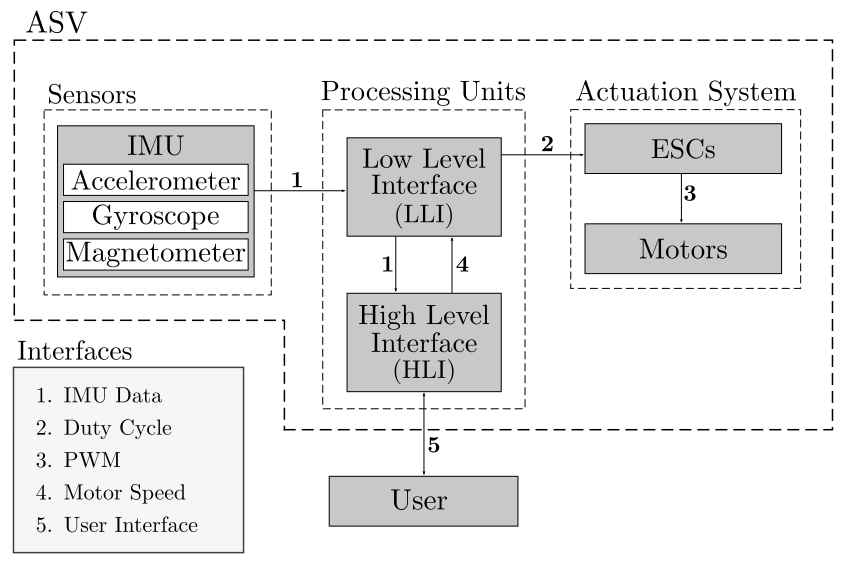
\includegraphics[width=.65\textwidth]{figures/systemDiagram4}
    \caption{Functional diagram of the given system.}
    \label{fig:systemDiagram}
\end{figure}
%
%The main parts of the system are the actuation system, the sensors and the processing units, see \autoref{fig:systemDiagram}. The processing unit gathers information from the IMU. This is handled by the Low Level Interface (LLI) which then sends it to the High Level Interface (HLI) where the control algorithms are implemented. The calculated actuation is then sent back to the LLI that sends the command to the actuation system. The ESCs (electronic speed controllers) then calculate the required signal to make the motors turn at the requested speed.

The main parts of the system are the actuation system, the sensors and the processing units, see \autoref{fig:systemDiagram}. The inertial measurement unit (IMU) information is gathered by the low level interface (LLI), and then transferred to the high level interface (HLI). In the HLI, the control algorithms are implemented, and the calculated commands are sent back to the actuation system through the LLI. The electronic speed controllers (ESCs) then calculate the required signal to make the motors turn at the requested speed.

This chapter briefly describes the main components of the surface vessel used in this project. Some additions to the existing systems are also presented.


    \section{Control System}\label{sec:ControlComputation}
\fxnote{Check the title os the section}

HLI - Computer( maybe wait until we know )

LLI - Arduino Interface to HLI bla bla


    \section{Actuators}

Forward and side thrusters

motors

ESCs

how to obtain a force on the actuators
    \section{Sensors}\label{sec:sensors}
The control system designed in the vessel requires the presence of sensor data that provides information about the vessel's motion. This is handled by an IMU.

The IMU installed in the vessel is formed by a triaxial gyroscope with a digital range scaling between $\pm300^{\circ}$ s$^{-1}$, a triaxial accelerometer with a range of $\pm$18 g and a triaxial magnetometer with a range of $\pm$\num{2.5} G. It also contains a serial peripheral interface (SPI) to obtain the data. \cite{IMUDatasheet}
%
\begin{figure}[H]
	\includegraphics[width=0.2\textwidth]{figures/IMU}
	\caption{ADIS16405BMLZ IMU module mounted in the vessel \cite{IMUFigure}}
	\label{fig:IMU}
\end{figure}
%
The data provided by the IMU is used to estimate both the position and the attitude of the vessel.

%Triaxial, digital gyroscope with digital range scaling
%±75°/sec, ±150°/sec, ±300°/sec settings
%Tight orthogonal alignment, 0.05°
%Triaxial, digital accelerometer, ±18 g
%Triaxial, digital magnetometer, ±2.5 gauss
%SPI-compatible serial interface
%Embedded temperature sensor
%Single-supply operation: 4.75 V to 5.25 V

%\subsection{GPS}
%The vessel has a UP-501 GPS Receiver installed. It operates with a update frequency up to 10 Hz and its trasmits the received position data through a serial communication to the Low Level Interface. \cite{GPS}
%
%\begin{figure}[H]
%	\includegraphics[width=0.3\textwidth]{figures/GPS}
%	\caption{UP-501 GPS receiver mounted in the vessel \cite{GPS}.}
%	\label{fig:GPS}
%\end{figure}
%%
%As the UP-501 is a standard GPS receiver, its precision is in the range of meters \fxnote{How to prove this?? Maybe make a test.}. This makes it cumbersome to control the position of the vessel using only GPS data, and thus, the GPS and the IMU data is combined to obtained the position of the vessel.
    \section{System Additions}
Some changes including GPS and communication setup are made, a full diagram is seen in \autoref{fig:systemDiagram2}.
%
\begin{figure}[H]
  \includegraphics[width=.65\textwidth]{figures/systemDiagram5}
  \caption{A functional diagram of the full system with additions.}
  \label{fig:systemDiagram2}
\end{figure}
%
The Real Time Kinematic GPS system, described in further detail below, is added to obtain better positioning of the ASV. This is necessary to obtain sub-meter positioning, without which the control design would have little impact on the performance of the system.\\
Additionally a VPN server and a USB modem is used to provide user input when the ASV and user are not on the same closed network. This makes it possible to access the ASV through the cellular network and thus eliminates potential problems with regards to range between user and ASV.

\section{Real Time Kinematic (RTK) GPS}
An RTK GPS system consists of two parts, a base station, and a rover.
The base station is set up at a stationary location with a known, precise GPS position.\\
The rover GPS, mounted on the ASV, measures its location, based on GPS satellites and measurements from the base station.\cite{EmlidRTK}\\
The module used in this project, both for the base and the rover GPS, is the Emlid Reach RTK GPS, see \autoref{fig:emlidReach}.

\begin{figure}[H]
  \includegraphics[width=0.27\textwidth]{figures/emlidReach}
  \caption{Emlid Reach RTK GPS module.\cite{EmlidReachDocs}}
  \label{fig:emlidReach}
\end{figure}

The base station gets its current position same as the rover using approximately the same satellites. Since the true position of the base is known, so is the error of each measurement. This is then sent as correction data to the rover, where the error is compensated for.%\cite{EmlidRTK}

An RTK GPS is able to archive a higher precision than an ordinary GPS by receiving correction data from a base station.
%The correction data is used by the rover to estimate signal disturbances, caused be the signals entering the atmosphere. 
This enables it to increase the precision of the GPS measurements, from 2-5m down to a theoretical precision of a few centimeters.\cite{EmlidRTK}

This data is formatted as an RTCM3 message, which is a protocol designed for this purpose.\\

\begin{figure}[H]
	\includegraphics[width=0.8\textwidth]{figures/comunicationSetup.pdf}
	\caption{Overall set up of GPS}
	\label{fig:rtk_GPS}
\end{figure}
%
\autoref{fig:rtk_GPS} shows how the RTK GPS system is set up. 
The computer runs a Python script which forwards the message to a TCP socket, making it accessible through the Internet. 
The HLI on the vessel connects to this socket and feeds the data to the Rover located on the boat.
For a more detailed description of the setup see \autoref{app:rtk_gps}.\fxnote{the reference should be to a test showing the iproved result of using a base for corrections}

    
    %---------- Chapter 4 ---------------------------------------- Modeling
    \chapter{System Model} \label{chap:model}
The model of the surface vessel is based in the methods presented in \cite{TFossen}, where the principal effects that affect the behavior of the vessel are taken into account are described in order to generate a model that serves as a basis for control design and simulations.\fxnote{write pages in the source}



    \section{Reference Frames}\label{sec:frames}
The attitude and position of the vessel is described using two coordinate frames, a body frame and an inertial frame. For operations in a local area, with longitude and latitude approximately constants (flat navigation) a NED system (North-East-Down) can be assumed as an inertial frame where Newtonian mechanics apply \cite[p. 17]{TFossen}.

To distinguish between the two frames, the body frame is denoted with a subindex "$_\mathrm{b}$", and the inertial frame with subindex "$_\mathrm{n}$". In \autoref{fig:refFrame}, a diagram of the surface vessel with the notation used can be seen.
\begin{figure}[H]
    \includegraphics[width=0.6\textwidth]{figures/boat3D}
    \caption{$x_\mathrm{b}$, $y_\mathrm{b}$ and $z_\mathrm{b}$ refer to the position with respect to the body coordinate frame, while $x_\mathrm{n}$, $y_\mathrm{n}$ and $z_\mathrm{n}$ describe it with respect to the inertial frame. $\phi$, $\theta$ and $\psi$ refer to the rotation around $x_\mathrm{b}$, $y_\mathrm{b}$ and $z_\mathrm{b}$, respectively.}
    \label{fig:refFrame}
\end{figure}

The transformation from the body frame to the inertial can be done through a rotation matrix, \eqref{eq:RotMatrix}, which describes a total rotation in terms of three consecutive rotations. Note that due to the size of the matrices sine and cosine are denoted $s$ and $c$ respectively.

In this case the rotation matrix is composed with a 1-2-3 convention, that is, first a rotation around $x_{\mathrm{b}}$, then around $y_{\mathrm{b}}$ and finally around $z_{\mathrm{b}}$ \cite[p. 22]{TFossen}.

\begin{minipage}{0.32\linewidth}
    \begin{flalign}
    \vec{R}_\mathrm{X} &=
    \begin{bmatrix}
    1 & 0      & 0       \\ 
    0 & c\phi  & -s\phi  \\ 
    0 & s\phi  & c\phi   \nonumber  
    \end{bmatrix}\ , 	\label{eq:RotMatrix1}
    \end{flalign}
\end{minipage}\hfill
\begin{minipage}{0.32\linewidth}
    \begin{flalign}
    \vec{R}_\mathrm{Y} &=
    \begin{bmatrix}
    c\theta  & 0  & s\theta  \\ 
    0          & 1  & 0      \\ 
    -s\theta & 0  & c\theta  \nonumber 
    \end{bmatrix}\ , 	\label{eq:RotMatrix2}
    \end{flalign}
\end{minipage}\hfill
\begin{minipage}{0.32\linewidth}
    \begin{flalign}
    \vec{R}_\mathrm{Z} &=
    \begin{bmatrix}
    c\psi & -s\psi  & 0  \\ 
    s\psi & c\psi   & 0  \\ 
    0       & 0         & 1  \nonumber 
    \end{bmatrix}\ , 	\label{eq:RotMatrix3}
    \end{flalign}
\end{minipage}\hfill
{\small
\begin{flalign}
\vec{R}^\mathrm{n}_\mathrm{b} = \vec{R}_Z \vec{R}_Y \vec{R}_X =
\begin{bmatrix}
c\theta c\psi  & s\phi s\theta c\psi -c\phi s\psi  & c\phi s\theta c\psi + s\phi s\psi  \\ 
c\theta s\psi  & s\phi s\theta s\psi + c\phi c\psi & c\phi s\theta s\psi - s\phi c\psi  \\ 
-s\theta         & s\phi c\theta                           & c\phi c\theta
\end{bmatrix} \ .	\label{eq:RotMatrix}
\end{flalign}}

%
\begin{where}
    \va{\vec{R}_\mathrm{X}}{is the matrix describing a rotation around the $x_\mathrm{b}$ axis}{}
    \va{\vec{R}_\mathrm{Y}}{is the matrix describing a rotation around the $y_\mathrm{b}$ axis}{}
    \va{\vec{R}_\mathrm{Z}}{is the matrix describing a rotation around the $z_\mathrm{b}$ axis}{}
    \va{\vec{R}^\mathrm{n}_\mathrm{b}}{is the total rotation matrix}{}
\end{where}

To describe a vector in the inertial frame given its description in the body frame, it is left multiplied by the rotation matrix as
%
\begin{flalign}
v_{\mathrm{n}}=\vec{R}^\mathrm{n}_\mathrm{b}v_\mathrm{b}\ . 
\end{flalign}
\begin{where}
    \va{v_{\mathrm{n}}}{is a column vector that contains the description with respect to the inertial frame}{}
    \va{v_{\mathrm{b}}}{is a column vector that contains the description with respect to the body frame}{}
\end{where}

If the inverse computation is needed, it is done following the same procedure using $\vec{R}^\mathrm{n\ T}_\mathrm{b}$ as the rotation matrix.    

\subsection{Rigid Body Dynamics}

The first step to model the motion of the surface vessel is to look at its rigid body dynamics. They are described assuming that the center of gravity of the boat coincides with the origin of the body coordinate frame.

The translational movement can be analyzed using Newton's second law, where the acceleration of the vessel is related to the applied forces as
%
\begin{flalign}
\sum F=m \ddot{x} \ .
\end{flalign}

For rotational movements, the motion is described using the Newton's second law applied to rotational movement, where the torques applied to the system influence the angular acceleration around each axis as
%
\begin{flalign}
\sum \tau=I \ddot{\theta}\ .
\end{flalign}

%The movement can be influence by the Coriolis effect, due to the fact that the body coordinate frame rotates with respect to the inertial frame. This effect, however, can be neglected in the case of a small vehicle that moves slow such as the vessel at hand \finite{find source}.
The rotational movement is affected by the Coriolis effect, which appears if the vessel is not rotating around the axis with least or highest inertial axis. However, the influence of this force is small if the vessel rotates at low speeds, hence it has been neglected in the model.  \cite[p. 170]{TFossen}

\section{Hydrostatics}
The hydrostatics describe what forces and torques are applied on the surface vessel by the volume of fluid displaced when floating on water. The force induced upon the vessel is called buoyancy force and it is applied to the center of buoyancy.  

The buoyancy force acts in the negative $z_\mathrm{n}$ direction as seen in
%
\begin{flalign}
B = \rho g (V + \Delta V(z))\ .
\end{flalign}
%
\begin{where}
    \va{\rho}{is the density of the fluid in which the vessel floats}{kg \cdot  m^{-3}}
    \va{g}{is the gravitational acceleration}{m \cdot s^{-2}}
    \va{V}{is the volume of fluid displaced by the surface vessel}{m^3}
    \va{\Delta V}{is the change in volume of fluid displaced by the surface vessel}{m^3}
    \va{B}{is the buoyancy force}{N}
\end{where}

When the vessel floats, the gravity force cancels out $ \rho g V $ of the buoyancy force, making the contribution of the latest along $x_\mathrm{b}$, $y_\mathrm{b}$ and $z_\mathrm{b}$ directions dependent only on the variation with respect to the equilibrium flotation point.
This result is seen in 
%
\begin{flalign}
F_{z_\mathrm{n}} = mg - \rho g V -\rho g  \Delta V(z) = -\rho g  \Delta V(z) \ .
\end{flalign}
\begin{where}
    \va{F_{z_\mathrm{n}}}{is the summation of forces along the $z_\mathrm{n}$ direction}{N}
\end{where}

The change in volume can be expressed as in \autoref{eq:deltaV}. The water plane of the vessel is not considered to vary significantly with change in vertical position, thus the approximation seen in the following equation is applied
%
\begin{flalign}
\Delta V(z) = \int_{0}^{z_\mathrm{N}}A_\mathrm{wp}(\zeta)d\zeta \approx A_\mathrm{wp}z_\mathrm{n} \ .
\label{eq:deltaV}
\end{flalign}
\begin{where}
    \va{A_\mathrm{wp}}{is the water plane area of the vessel}{m^2}
\end{where}

The contribution along the body frame directions is calculated as a function of the $\phi$ and $\theta$ angles in  
%
\begin{flalign}
F_{x_\mathrm{b}} &= -\rho g A_\mathrm{wp}z_\mathrm{n} (-\sin \theta)  \ , \\
F_{y_\mathrm{b}} &= -\rho g A_\mathrm{wp}z_\mathrm{n} (\cos \theta \sin   \phi) \ , \\
F_{z_\mathrm{b}} &= -\rho g A_\mathrm{wp}z_\mathrm{n} (\cos \theta \cos  \phi) \ .
\label{eq:forcez}
\end{flalign}

%If the variations of $\phi$ and $\theta$ are small, the contribution of the buoyancy force in the $x_\mathrm{b}$ and $y_\mathrm{b}$ directions can be neglected and not included in the final model of the vessel. \cite[pp. 62-67]{TFossen}

The buoyancy force also contributes with some torques around the different axis in the body coordinate frame. This occurs as the center of buoyancy in general is not aligned with the center of gravity, generating some restoring torques on the vessel. These are dependent on the gravity and the buoyancy force. As the contribution of the term $\rho g \Delta V$ is small compared to that of $\rho g V$, only the latter is considered in the model \cite[pp. 62-67]{TFossen}. These torques are expressed as
%
\begin{flalign}
T_{\phi} &= -\rho g V \overline{GM}_{\mathrm{T}} \sin \phi (\cos \theta \cos \phi)   \ ,
\label{eq:torqphi} \\
T_{\theta} &= -\rho g V \overline{GM}_{\mathrm{L}} \sin \theta (\cos \theta \cos \phi) \ .
\label{eq:torqtheta}
\end{flalign}
\begin{where}
    \va{T_{\phi}}{is the restoring torque due to the buoyancy force in the $\phi$ direction}{N \cdot m}
    \va{T_{\theta}}{is the restoring torque due to the buoyancy force in the $\theta$ direction}{N \cdot m}
    \va{\overline{GM}_\mathrm{T}}{is the transverse metacentric height}{m}
    \va{\overline{GM}_\mathrm{L}}{is the longitudinal metacentric height}{m}
\end{where}

The metacentric heights are the distances between the center of gravity and the metacenter of the vessel. The metacenter position the intersection of imaginary vertical lines that go through the different centers of buoyancy originated when tilting or displacing the vessel. This height can be seen in \autoref{fig:app_metacentric}.

\begin{figure}[H]
    %\includegraphics[width=0.5\textwidth]{figures/app_metacentric}
    \caption{\cite[p. 62]{TFossen} \fxnote{include figure from book}}
    \label{fig:app_metacentric}
\end{figure}

\section{Hydrodynamics}
The hydrodynamic forces induced in the surface vessel are mainly caused by two terms. The added mass and the viscous damping.

The added mass induces a force that originate from the vessel imposing some energy in the surrounding fluid when the vessel moves through it, which is dependent on the acceleration of the vessel. However, this effect is neglected since most of the effective mass of the vessel comes from the nominal mass, and any variation is handled by the controller.

The viscous damping is a combination of several factors, namely, skin friction, wave drift damping and vortex shedding \cite[p. 122]{TFossen}. This type of damping appears in the equations as coefficients that multiply, with negative sign, the different translational and angular velocities that define the movement of the vessel. For each degree of freedom it is expressed as
%
\begin{flalign}
D_{\dot{x}_\mathrm{b}} &= - d_{\dot{x}_\mathrm{b}}  \dot{x}_\mathrm{b}\ , \\
D_{\dot{y}_\mathrm{b}} &= - d_{\dot{y}_\mathrm{b}}  \dot{y}_\mathrm{b}\ , \\
D_{\dot{z}_\mathrm{b}} &= - d_{\dot{z}_\mathrm{b}}  \dot{z}_\mathrm{b}\ , \\
D_{\dot{\phi}} &= - d_{\dot{\phi}}                  \dot{\phi}\ , \\
D_{\dot{\theta}} &= - d_{\dot{\theta}}              \dot{\theta}\ , \\
D_{\dot{\psi}} &= - d_{\dot{\psi}}                  \dot{\psi}\ .  \\
\end{flalign}
\begin{where}
    \va{D_{i}}{is the damping force or torque due to viscous damping}{N, \ N \cdot m}
    \va{d_{i}}{is the viscous damping coefficient}{N \cdot m^{-1} \cdot s, \ N \cdot m \cdot rad^{-1} \cdot s}
\end{where}

These equations consider that the viscous friction is linear, since this assumption can be done for vessel speeds lower than 2 m/s \cite[p. 138]{TFossen}. 

    \section{Model Equations}   
The final model equations are presented in this section.
The model equations will be presented, linarized and put into state space.
\autoref{fig:boat3DForces} and \ref{fig:boat2D} show a diagram of the vessel.
The model equations are presented in to body frame, meaning all movement is relative to the boat. 
The states can be transformed into the inertial frame, using equation \autoref{eq:RotMatrix}.  
\begin{figure}[H]
    \captionbox  %<--use captionbox instead if no global caption is needed
    {               %                                \%-%-%-%-%-%-%\
        Diagram of the boat where the forces applied by the motors are shown.                %\
        \label{fig:boat3DForces}                                  %\
    }                                                                 %\
    {                                                                  %\
        \includegraphics[width=.46\textwidth]{figures/boat3DForces}         %\
    }                                                                    %\
    \hspace{5pt}                                                          %\
    \captionbox  %<-----------------------------------------------------%\
    {       
        Above perspective of the vessel, where the distances needed for the model equations are presented.                                                                %\                         %\
        \label{fig:boat2D}                                     %\
    }                                                                           %\
    {                                                                            %\
        \includegraphics[width=.2\textwidth]{boat2D}            %|
    }                                                                             %|
\end{figure}
%
The translational movement of the vessel is described by \autoref{eq:x_pos_model}, \ref{eq:y_pos_model} and \ref{eq:z_pos_model}.
The model relates the forces applied by the motors to the boat frame. 
%
\begin{flalign}
	m_\mathrm{x} \ddot{x}_\mathrm{b} &=  F_\mathrm{1} + F_\mathrm{2}  - d_{\dot{x}_\mathrm{b}} \dot{x}_\mathrm{b} + F_{x_\mathrm{b}}
    \label{eq:x_pos_model} \\
    m_\mathrm{y} \ddot{y}_\mathrm{b} &=  -d_{\dot{y}_\mathrm{b}} \dot{y_\mathrm{b}} + F_{y_\mathrm{b}}
    \label{eq:y_pos_model} \\
    m_\mathrm{z} \ddot{z}_\mathrm{b} &=  -d_{\dot{z}_\mathrm{b}}\dot{z_\mathrm{b}} + F_{z_\mathrm{b}} \label{eq:z_pos_model}
\end{flalign}
%
\begin{where}
	\va{m_\mathrm{x,y,z}}{Is the virtual mass in their respective direction}{kg}
%    \va{m_\mathrm{x}}{}{kg}
%    \va{m_\mathrm{y}}{}{kg}
%    \va{m_\mathrm{z}}{}{kg}
    \va{\ddot{x}_\mathrm{b}}{is the acceleration in the $x_\mathrm{b}$ direction}{m s^{-2}}
    \va{\ddot{y}_\mathrm{b}}{is the acceleration in the $y_\mathrm{b}$ direction}{m s^{-2}}
    \va{\ddot{z}_\mathrm{b}}{is the acceleration in the $z_\mathrm{b}$ direction}{m s^{-2}}
    \va{\dot{x}_\mathrm{b}}{is the velocity in the $x_\mathrm{b}$ direction}{m s^{-1}}
    \va{\dot{y}_\mathrm{b}}{is the velocity in the $y_\mathrm{b}$ direction}{m s^{-1}}
    \va{\dot{z}_\mathrm{b}}{is the velocity in the $z_\mathrm{b}$ direction}{m s^{-1}}
    \va{F_1}{is the force applied by motor 1}{N}
    \va{F_2}{is the force applied by motor 2}{N}
\end{where} \\
% 
From the equations it shows that only the x-axis on the boat frame is controllable, as this is the axis containing the main thrusters. 
While the vessel do contain side thrusters, they are only intended for fine maneuvering, as their strength is relatively weak, compared to the main thrusters.\\
%
The virtual mass components is the added mass from the displaced water in the respective direction plus the mass of the vessel.
This value will be different for each axis, as the difference in shape drags a different amount of water with it depending on the direction.
    
The angular movement of the vessel is described by \autoref{eq:phi_model}, \ref{eq:theta_model} and \ref{eq:psi_model}.

\begin{flalign}
    I_\mathrm{x}\ddot{\phi} &= -d_{\dot{\phi}} \dot{\phi} + T_\mathrm{\phi}  
    \label{eq:phi_model} \\
    I_\mathrm{y}\ddot{\theta} &= -d_{\dot{\theta}} \dot{\theta} + T_\mathrm{\theta}  
    \label{eq:theta_model} \\
    I_\mathrm{z}\ddot{\psi} &= F_\mathrm{1}l_\mathrm{1} - F_\mathrm{2} l_\mathrm{2} - d_{\dot{\psi}} \dot{\psi} \label{eq:psi_model}
\end{flalign}
%
\begin{where}
    \va{I_\mathrm{x}}{is the inertia around the $x_\mathrm{b}$ axis}{kg}
    \va{I_\mathrm{y}}{is the inertia around the $y_\mathrm{b}$ axis}{kg}
    \va{I_\mathrm{z}}{is the inertia around the $z_\mathrm{b}$ axis}{kg}
    \va{\ddot{\phi}}{is the angular acceleration around the $x_\mathrm{b}$ axis}{rad s^{-2}}
    \va{\ddot{\theta}}{is the angular acceleration around the $y_\mathrm{b}$ axis}{rad s^{-2}}
    \va{\ddot{\psi}}{is the angular acceleration around the $z_\mathrm{b}$ axis}{rad s^{-2}}
    \va{\dot{\phi}}{is the angular velocity around the $x_\mathrm{b}$ axis}{rad s^{-1}}
    \va{\dot{\theta}}{is the angular velocity around the $y_\mathrm{b}$ axis}{rad s^{-1}}
    \va{\dot{\psi}}{is the angular velocity around the $z_\mathrm{b}$ axis}{rad s^{-1}}
    \va{l_1}{is the perpendicular distance from motor 1 to the center of gravity}{m}
    \va{l_2}{is the perpendicular distance from motor 2 to the center of gravity}{m}
\end{where}

Similar to the translatoric equations, only one axis is controllable, due to the lack of actuators. 
This will not be a problem in practice, as yaw is the only direction that it desirable to control, and any torque induced upon the other axis is a be product of the dynamics.

    \section{Linearization of Model Equations}\label{sec:linearizationModel}
The model equations need to be linearized to be able to design a controller using linear techniques. This is done using the first order Taylor approximation around an equilibrium as seen in 
\begin{flalign}
    f(x) &\approx f(\overline{x}) + f'(\overline{x}) (x-\overline{x})  \rightarrow\ \tilde{f}(x) \approx f'(\overline{x}) \tilde{x}
    \label{taylor}
\end{flalign}
In this equation, $\overline{x}$ represents the equilibrium point and $\tilde{x}$ the equilibrium point.

The equilibrium point must fulfill that all the derivatives of the states are zero, in this case the velocities and accelerations. This also result in the restoring forces and torques, as well as the motor forces equal to zero. 

To apply the approximation, the function must be differentiated with respect to each of the present variables, and once linearized, the function is expressed in terms of variations from the equilibrium point.
%
\begin{flalign}
    f &= f(x_1,x_2,...,x_\mathrm{n}) \nonumber \\
    \tilde{f}&=\frac{\partial f}{\partial x_1}\bigg|_{\overline{x}_1,\overline{x}_2,...,\overline{x}_n}\ \tilde{x}_1 + \frac{\partial f}{\partial x_2}\bigg|_{\overline{x}_1,\overline{x}_2,...,\overline{x}_n}\ 
    \tilde{x}_2+...+ \frac{\partial f}{\partial x_n}\bigg|_{\overline{x}_1,\overline{x}_2,...,\overline{x_n}}\ \tilde{x}_\mathrm{n} \nonumber
    \label{eq:dummytaylor}
\end{flalign}

In the case of the boat, the only non-linear terms are the restoring forces and torques. They can be linearized and give the result seen in 
%
\begin{flalign}
    \tilde{F}_{x_\mathrm{b}} &= 0  \label{eq:forcexlin}\\
    \tilde{F}_{y_\mathrm{b}} &= 0  \label{eq:forceylin}\\
    \tilde{F}_{z_\mathrm{b}} &= -\rho g A_\mathrm{wp} \tilde{z}_\mathrm{n} \label{eq:forcezlin} \\
 	\tilde{T}_{\phi} &= -\rho g V \overline{GM_{L}}\cdot \tilde{\phi} \label{eq:torquephilinar} \\
    \tilde{T}_{\theta} &= -\rho g V \overline{GM_{L}}\cdot \tilde{\theta}\label{eq:torquethetalinar}   
\end{flalign}

The first order Taylor approximation is only applicable in areas close to the operating point, however as the vessel should not deviate much from this during operation. 

From now on, the linearized variables are represented without the symbol $\Delta$, to avoid excessive notation, even though they refer to changes with respect to the the equilibrium point.

The model equations including these linearized terms end up being
%
\begin{flalign}
 	m_\mathrm{x} \ddot{x}_\mathrm{b} &=  F_\mathrm{1} + F_\mathrm{2}  - d_{\dot{x}_\mathrm{b}} \dot{x}_\mathrm{b}
     \label{eq:x_pos_model_lin} \\
    m_\mathrm{y} \ddot{y}_\mathrm{b} &=  -d_{\dot{y}_\mathrm{b}} \dot{y_\mathrm{b}}
     \label{eq:y_pos_model_lin} \\
    m_\mathrm{z} \ddot{z}_\mathrm{b} &=  -d_{\dot{z}_\mathrm{b}}\dot{z_\mathrm{b}} -\rho g A_\mathrm{wp} \tilde{z}_\mathrm{n} \label{eq:z_pos_model_lin}   \\
    I_\mathrm{x}\ddot{\phi} &= -d_{\dot{\phi}} \dot{\phi} - \rho g V \overline{GM_{L}}\cdot \tilde{\phi} 
    \label{eq:phi_model_limn} \\
    I_\mathrm{y}\ddot{\theta} &= -d_{\dot{\theta}} \dot{\theta} - \rho g V \overline{GM_{L}}\cdot \tilde{\theta} 
    \label{eq:theta_model_lin} \\
    I_\mathrm{z}\ddot{\psi} &= F_\mathrm{1}l_\mathrm{1} - F_\mathrm{2} l_\mathrm{2} - d_{\dot{\psi}} \dot{\psi} \label{eq:psi_model_lin}
\end{flalign}



%\begin{flalign}
%    m_\mathrm{x} \ddot{x}_\mathrm{b} &=  F_\mathrm{1} + F_\mathrm{2}  - d_\mathrm{x} \dot{x}_\mathrm{b} + m_\mathrm{y} \dot{y_\mathrm{b}} \dot{\psi} - m_\mathrm{z} \dot{z}_\mathrm{b} \dot{\theta} - F_\mathrm{x}
%    \label{eq:x_pos_model} \\
%    m_\mathrm{y} \ddot{y_\mathrm{b}} &=  -d_\mathrm{y}\dot{y_\mathrm{b}}-m_\mathrm{x}\dot{x_\mathrm{b}}\dot{\psi}+m_\mathrm{z}\dot{z_\mathrm{b}}\dot{\phi}-F_\mathrm{y}
%    \label{eq:y_pos_model} \\
%    m_\mathrm{z} \ddot{z_\mathrm{b}} &=  -d_\mathrm{z}\dot{z_\mathrm{b}}+ m_\mathrm{b}\dot{x_\mathrm{b}}\dot{\theta}-m_\mathrm{y}\dot{y_\mathrm{b}} \dot{\phi}-F_\mathrm{z} \label{eq:z_pos_model}
%\end{flalign}
%
%\begin{flalign}
%    I_\mathrm{x}\ddot{\phi} &= -d_\mathrm{\phi} \dot{\phi}-(m_\mathrm{z}-m_\mathrm{y}) \dot{z}_\mathrm{b} \dot{y}_\mathrm{b}-(I_\mathrm{z}-I_\mathrm{y}) \dot{\theta } \dot{\psi}+T_\mathrm{\phi}  
%    \label{eq:x_inert_model} \\
%    I_\mathrm{y}\ddot{\theta} &= -d_\mathrm{\theta} \dot{\theta}-(m_\mathrm{z}-m_\mathrm{x}) \dot{x}_\mathrm{b} \dot{y}_\mathrm{b}-(I_\mathrm{x}-I_\mathrm{z}) \dot{\phi} \dot{\psi}+T_\mathrm{\theta}  
%    \label{eq:y_inert_model} \\
%    I_\mathrm{z}\ddot{\psi} &= -d_\mathrm{\psi} \dot{\psi}-(m_\mathrm{y}-m_\mathrm{x}) \dot{x}_\mathrm{b}\dot{y}_\mathrm{b}-(I_\mathrm{z}-I_\mathrm{y})\dot{\psi}\dot{\theta}+F_\mathrm{1}l_\mathrm{1}+F_\mathrm{2}l_\mathrm{2}+T_\mathrm{\psi} \label{eq:z_inert_model}
%\end{flalign}

    \section{Model Verification}\label{sec:modelVerification}
   

    %%% PART 2 %%%
    \part{Design}
    %---------- Chapter 5 ---------------------------------------- Design Approach
    \chapter{Design Approach}
\begin{figure}[H]
    \includegraphics[width=0.3\textwidth]{figures/controllerDiagram2}
    \caption{}
    \label{fig:controllerDiagram}
\end{figure}
    %---------- Chapter 7 ---------------------------------------- Controller Design
    \chapter{Inner Controller Design}

Header of control chapter

\begin{figure}[H]
    \includegraphics[width=0.8\textwidth]{figures/controllerDiagram}
    \caption{}
    \label{fig:controllerDiagram}
\end{figure}
    \section{Initial Control Design}
%
It is desired to design a state feedback using a linear quadratic regulator (LQR). As the controller eventually must be implemented the design is carried out in the discrete domain. To do so, it is necessary to discretize the system. A discrete state space model can be expressed as,
%
\begin{flalign}
  \vec{x}(k+1) &= \vec{A_z} \vec{x}(k) + \vec{B_z} \vec{u}(k)
  \label{xDotLinearDiscrete} \\
  \vec{y}(k)   &= \vec{C_z} \vec{x}(k) + \vec{D_z} \vec{u}(k) \ \ ,
  \label{yLinearDiscrete} 
\end{flalign}
%
where the z subindexes indicate the matrices being in the discrete domain and k is the sample index. The model is discretized using zero order hold. In \autoref{fig:discreteSSBlock} the discrete system is shown in a block diagram. The feed forward matrix is excluded as it is not present in this system.
%
\begin{figure}[H]
  \includegraphics[width=0.6\textwidth]{figures/discreteSystemBlockDiagram}
  \caption{Block diagram of the discrete system without feed forward.}
  \label{fig:discreteSSBlock}
\end{figure}
%
\fxnote{talk about controllability here.}
%
In order to track a reference and handle input disturbances, it is chosen to also include an integral controller in the design. The final control structure is seen in \autoref{fig:blockConrolDesignLQR}.
%
\begin{figure}[H]
  \includegraphics[width=0.9\textwidth]{figures/integralControlBlockDiagram}
  \caption{Block diagram of the control structure in the discrete domain.}
  \label{fig:blockConrolDesignLQR}
\end{figure}
%
To design this feedback system, it is convenient to express it on the following form:
\begin{flalign}
  \vec{x_e}(k+1) &= \vec{A_e} \vec{x}(k) + \vec{B_e} \vec{u}(k) + \vec{r}(k)
  \label{eq:xDotLinearDiscrete} \\
  \vec{y}(k)     &= \vec{C_e} \vec{x}(k)  \ \ .
  \label{eq:yLinearDiscrete} 
\end{flalign}
%
To describe the control design in this form, the $\vec{A_e}$, $\vec{B_e}$ and $\vec{C_e}$ matrices must be constructed. From \autoref{fig:blockConrolDesignLQR}, following relation is found:
%
\begin{flalign}
  \vec{x_I}(k+1) &= \vec{x_I}(k) + \vec{y}(k) + \vec{r}(k)    \nonumber \\
  \vec{x_I}(k+1) &= \vec{x_I}(k) - C_z \vec{x}(k) + \vec{r}(k)  \ \ .
  \label{eq:xIDiscrete}
\end{flalign}
%
This leads to the discrete state space model extended with the integral state expressed as
%
\begin{flalign}
  \begin{bmatrix}
    \vec{x}(k+1)  \\
    \vec{x_I}(k+1)
  \end{bmatrix}
  =
  \begin{bmatrix}
    \vec{A}_{\vec{z}_{3x3}} & \vec{O}_{_{3x2}} \\
   -\vec{C}_{\vec{z}_{2x3}} & \vec{I}_{_{2x2}} \\
  \end{bmatrix}
  \begin{bmatrix}
    \vec{x}(k)    \\
    \vec{x_I}(k)
  \end{bmatrix}
  +
  \begin{bmatrix}
    \vec{B}_{\vec{z}_{3x2}} \\
    \vec{O}_{2x2}
  \end{bmatrix}
  \vec{u}(k)
  +
  \begin{bmatrix}
    \vec{O}_{3x2} \\
    \vec{I}_{2x2}
  \end{bmatrix}
  \vec{r}(k)
  \label{eq:discreteSSWithIntegralX}
\end{flalign}  
%
\begin{flalign}
  \vec{y}(k)
  =
  \begin{bmatrix}
    \vec{C}_{\vec{z}_{2x3}} &  \vec{O}_{2x2}
  \end{bmatrix}
  \begin{bmatrix}
    \vec{x}(k)    \\
    \vec{x_I}(k)
  \end{bmatrix}  \ \ ,
  \label{eq:discreteSSWithIntegralY}
\end{flalign}  
%
which cooresponds to \autoref{eq:xDotLinearDiscrete} and \ref{eq:yLinearDiscrete}.

A discrete time infinite horizon LQR is used in the design of the feedback, $\vec{F_e} = [\ \vec{F} \ \ \vec{F}_\mathrm{I} ]\ $, which works by minimizing the cost function,
%
\begin{flalign}
  J = \sum_{k=0}^\infty \vec{x}_k^\mathrm{T}\vec{Q}\vec{x}_k + \vec{u}_k^\mathrm{T}\vec{R}\vec{u}_k \ dt \ \ .
\end{flalign}
\begin{where}
	\va{\vec{Q}}{is the state cost matrix}{}
  \va{\vec{R}}{is the input cost matrix}{}
\end{where}

The Q matrix contains the penalties for the state, such that a higher cost is generated for more critical states, thus driving these states faster to zero. The R matrix contains the penalties for the input. This helps to ensure that the actuators never enters saturation.
Bryson's rule is used to determine sensible values for the state and input penalties in the Q and R matrices.
%
\begin{flalign} 
Q_{ii} &= \frac{1}{[x_{i_\mathrm{max}}]^2} \ \ \ \ R_{ii} = \frac{1}{[u_{i_\mathrm{max}}]^2}
\label{eq:QRBryson}
\end{flalign}
\begin{where}
  \va{x_{i_\mathrm{max}}}{are the maximum acceptable state values}{}
  \va{u_{i_\mathrm{max}}}{are the maximum acceptable input values}{}
\end{where}

From this the state feedback is calculated by,
%
\begin{flalign} 
  \vec{F}_\mathrm{e} &= (\vec{R} \vec{B}_\mathrm{e}^\mathrm{T} \vec{P}\vec{B}_\mathrm{e})^{-1}  \vec{B}_\mathrm{e}^\mathrm{T} \vec{P}\vec{B}_\mathrm{e}
  \label{eq:QRFeedback}
\end{flalign}
\begin{where}
  \va{\vec{P}}{is the state transfer matrix.}{}
\end{where}

$\vec{P}$ provides a feedback matrix which minimizes the cost function, and can be found by use of the Riccatti equation.
%$\vec{F}_\mathrm{e}$ can be seperated to make F and F_I as the first 6 columns are state feedback and the last three are the integral control. These feedback matricees can can be implemented as shown in \autoref{fig:blockConrolDesignLQR}.












    %\subsection{Controller Performance}
The performance of the controller can be seen in \autoref{fig:xbdot_lqr} and \ref{fig:yaw_lqr}. 
\begin{figure}[H]
    \captionbox 
    {   
        Step response of the model with linear quadratic regulator in $\dot{x}_\mathrm{b}$.
        \label{fig:xbdot_lqr}
    }                                                                 
    {                                                                  
        \includegraphics[width=.45\textwidth]{figures/xbdot_lqr}         
    }                                                                    
    \hspace{5pt}                                                          
    \captionbox  
    {      
        Step response of the model with the linear quadratic regulator in $\psi$ at 10 s.
        \label{fig:yaw_lqr}
    }                                                                          
    {
        \includegraphics[width=.45\textwidth]{figures/yaw_lqr}
    }
\end{figure}
%
In the simulation, a step reference is set to $\dot{x}_\mathrm{b}$ and then a reference is set to $\psi$ at 10 s. This is done to analyze the behavior closed ot real conditions, when the boat is turning while having constant speed.

It can be seen in \autoref{fig:xbdot_lqr} that the settling time, with an error band of 5 \%, for $\dot{x}_\mathrm{b}$ is around \num{0.5} s. There is not overshoot until the response is disturbed when the reference for $\psi$ is set, but it recovers in less than \num{0.2} s.

The response in $\psi$, \autoref{fig:yaw_lqr}, has a settling time of \num{2.2} s and an overshoot of less than 5 \%.

\fxnote{Check seconds and settling times with final graphs in LQR simulations}
    \section{$\mathcal{H}_\infty$ Design}\label{sec:Hinf}
The model in \autoref{sec:linearizationModel} has varying parameters, such as the mass or damping coefficients. The vessel may also experience external disturbances, such as wind, wave or current forces. During surveying, it is convenient for the vessel to be robust to these model variations and it must be able to sufficiently reject disturbances. Using the $\mathcal{H}_\infty$ design technique, a robust controller for the vessel can be synthesized. In this case, the design of model and controller is done simultaneously and can not be as clearly separated as for the LQR.

The $\mathcal{H}_\infty$ problem is solved by finding an internally stabilizing controller that provides a closed loop $\mathcal{H}_\infty$ norm less than some bound, $\gamma$, \cite[p. 835]{JCDoyle}, \cite[pp. 92-93]{AAStoorvogel}. Such a controller is also called suboptimal $\mathcal{H}_\infty$ controller, as there might be smaller $\gamma$ yielding an internally stabilizing controller.% The reason for not deigning the optimal controller is \fxnote{write reason}

A more detailed mathematical formulation of the $\mathcal{H}_\infty$ problem and its solution is given in \cite[pp. 91-119]{AAStoorvogel}. 

The state space model from \autoref{xDotLinear} and \autoref{yLinear} needs to be remodeled into a state space form suitable for solving the suboptimal $\mathcal{H}_\infty$ control problem \cite[pp. 95]{AAStoorvogel}, \cite[p. 64]{robustNotes}. This form is
\begin{flalign}
  \vec{\dot{x}}_\infty(t) &= \vec{A}_1 \vec{x}_\infty(t) + \vec{B}_1 \vec{w}(t) + \vec{B}_2 \vec{u}(t)\ ,
  \label{eq:xDotHinf} \\
  \vec{z}(t) &= \vec{C}_1 \vec{x}_\infty(t) + \vec{D}_{11} \vec{w}(t) + \vec{D}_{12} \vec{u}(t)\ ,
  \label{eq:zHinf} \\
  \vec{y}_\infty(t) &= \vec{C}_2 \vec{x}_\infty(t) + \vec{D}_{21} \vec{w}(t) + \vec{D}_{22} \vec{u}(t)\ ,
  \label{eq:yHinf} 
\end{flalign}
\begin{where}
  \va{\vec{x}_\infty}{is the state vector}{}
  \va{\vec{w}}{is the uncontrolled input vector}{}
  \va{\vec{u}}{is the controlled input vector}{}
  \va{\vec{z}}{is the performance output vector}{}
  \va{\vec{y}_\infty}{is the measured output vector}{}
  \va{\vec{A}_1}{is the state matrix}{}
  \va{\vec{B}_1}{is the uncontrolled input matrix}{}
  \va{\vec{B}_2}{is the controlled input matrix}{}
  \va{\vec{C}_1}{is the performance output matrix}{}
  \va{\vec{D}_{11}}{is the direct feedforward matrix from $\vec{w}$ to $\vec{z}$}{}
  \va{\vec{D}_{12}}{is the direct feedforward matrix from $\vec{u}$ to $\vec{z}$}{}
  \va{\vec{C}_2}{is the measured output matrix}{}
  \va{\vec{D}_{21}}{is the direct feedforward matrix from $\vec{w}$ to $\vec{y}_\infty$}{}
  \va{\vec{D}_{22}}{is the direct feedforward matrix from $\vec{u}$ to $\vec{y}_\infty$}{}
\end{where}

The $\mathcal{H}_\infty$ model representation can also be seen in \autoref{fig:HinfDiag}, where all signals and matrices involved in the design process are represented.
\begin{figure}[H]
	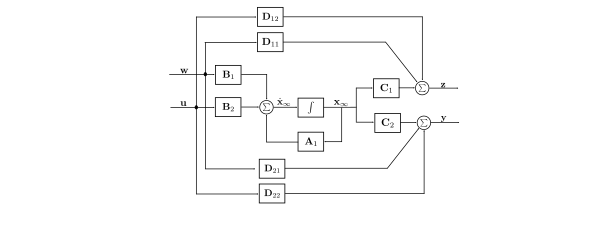
\includegraphics[width=0.6\textwidth]{figures/HinfDiag}
	\caption{Block diagram used in the $\mathcal{H}_\infty$ controller design.}
	\label{fig:HinfDiag}
\end{figure}

The method used to achieve the solution to the problem requires assuming certain conditions on the matrices in the model \cite[p. 835]{JCDoyle}. These conditions are 
\begin{enumerate}
	\item $\left (\vec{A}_1,\vec{B}_1 \right)$ and $\left( \vec{A}_1, \vec{B}_2 \right)$ are stabilizable.
	\item $\left (\vec{C}_1,\vec{A}_1 \right)$ and $\left( \vec{C}_2, \vec{A}_1 \right)$ are detectable.
	\item $\vec{D}_{12}^\mathrm{T}[\vec{C}_1\ \vec{D}_{12}]$ is $[\vec{0}\ \vec{I}]$.
	\item $\begin{bmatrix}
				\vec{B}_1 \\
				\vec{D}_{21} 
			\end{bmatrix}\vec{D}_{21}^\mathrm{T}$ is $[\vec{0}\ \vec{I}]$.
	\item $\vec{D}_{11}$ and $\vec{D}_{22}$ are zero.
\end{enumerate}

For obtaining the matrices present in \autoref{eq:xDotHinf}, \ref{eq:zHinf} and \ref{eq:yHinf}, the content of the state vector and signal vectors needs to be defined.

\subsection{State Vector}
The state vector construction starts with the three states that define the basic dynamics of the system. Namely, $\psi$, $\dot{\psi}$ and $\dot{x}_\mathrm{b}$. As some reference tracking is desired, integral states need to be included in the state vector, these depend on the measured output and the reference signal as 
\begin{flalign}
	\vec{\dot{x}}_\mathrm{I}(t) =
	\begin{bmatrix}
		x_{\mathrm{I}_{\psi}} \\
		x_{\mathrm{I}_{\dot{x}_\mathrm{b}}}
	\end{bmatrix}\ = 
	\begin{bmatrix}
		\psi_\mathrm{ref}-\psi \\
		\dot{x}_\mathrm{b,ref} - \dot{x}_\mathrm{b}
	\end{bmatrix}\ .
	\label{eq:xintVectorHinf}
\end{flalign}

The state vector also includes the states coming from the reference, disturbance and noise models. These extra states show the dynamics of the uncontrolled inputs, to which some weighting functions are applied. This process is carried out in order to modify how the uncontrolled inputs affect the states, and this is normally done through transfer functions, \cite{MSalari}. In order to include weights in the state space representation, some states for each uncontrolled input need to be defined. \autoref{fig:WeightDiag} shows an example of how an uncontrolled input is weighted so it can be included in the state space representation.
\begin{figure}[H]
	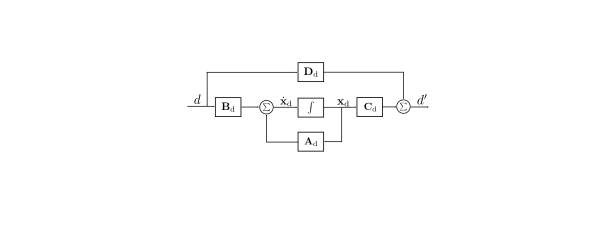
\includegraphics[width=0.6\textwidth]{figures/WeightDiag}
	\caption{Block diagram illustrating how an uncontrolled input is weighted in the $\mathcal{H}_\infty$ controller design. $d$ is the uncontrolled input and $d'$ is the weighted uncontrolled input. The states $\vec{x}_\mathrm{d}$ are included in the state vector of the $\mathcal{H}_\infty$ state space representation.}
	\label{fig:WeightDiag}
\end{figure}

The $\vec{A}_\mathrm{d}$, $\vec{B}_\mathrm{d}$, $\vec{C}_\mathrm{d}$ and $\vec{D}_\mathrm{d}$ in \autoref{fig:WeightDiag} can be calculated from a weighting function as in the example given in \autoref{eq:weightingexampleLP}, where the uncontrolled input $d$ is weighted by means of a first order transfer function with low pass characteristics.
\begin{flalign}
	\frac{d'}{d}=\frac{a}{s+a} \rightarrow \dot{d}' = -a d' + a d \rightarrow \begin{cases} \dot{x}_\mathrm{d} = -a x_\mathrm{d} + a d \\ d' = x_\mathrm{d} \end{cases}\label{eq:weightingexampleLP} 
\end{flalign}
\begin{where}
	\va{a}{is a parameter defining the pole position of the weighting function}{}
\end{where}
Another example with a high pass weighting function is shown in \autoref{eq:weightingexampleHP}.
\begin{flalign}
	\frac{n'}{n}=\frac{s}{s+a} = \frac{-a}{s+a}-1 \rightarrow \begin{cases} \dot{x}_\mathrm{n} = -a x_\mathrm{n} + n \\ n' = - a x_\mathrm{n} + n  \end{cases}\label{eq:weightingexampleHP} 
\end{flalign}
%
This process also entails defining the weights for each uncontrolled input. The weight on the reference is set to be a first order transfer function with a very fast pole so the step input does not get distorted. The weights on the input disturbances are also low pass filtered as most of them appear at low frequencies.

The noise, on the other hand, is weighted according to a high pass filter, as it is stronger in the high frequency range. In this way, the controller design focuses on achieving a robust controller with respect to the uncontrolled inputs in their particular frequency ranges. The chosen frequencies are 1, 20 and 20 rad$\cdot$s$^{-1}$ for the references, wind, current and wave disturbances low pass filters, respectively, and 100 rad$\cdot$s$^{-1}$ for the noise high pass filter. The reference frequency is used as a tuning parameter. The disturbances frequencies are calculated to be more conservative than the value obtained in \autoref{app:Disturbance}, while the noise frequency is assumed to be present as higher frequency than 100 rad$\cdot$s$^{-1}$. The weights for each uncontrolled input are

\begin{minipage}{0.49\linewidth}
\begin{flalign}
	W_{\psi_\mathrm{ref}} &= \frac{1}{s+1}\ ,\nonumber \\
	W_{F_\mathrm{wc}} &= \frac{20}{s+20}\ ,\nonumber\\
	W_{F_\mathrm{wave}} &= \frac{20}{s+20}\ ,\nonumber\\
	W_{n_\psi} &= \frac{s}{s+100}\ ,\nonumber
\end{flalign}
\end{minipage}
\begin{minipage}{0.49\linewidth}
\begin{flalign}
	W_{\dot{x}_\mathrm{b,ref}} &= \frac{1}{s+1}\ ,\nonumber \\
	W_{\tau_\mathrm{wc}} &= \frac{20}{s+20}\ , \nonumber\\
	W_{\tau_\mathrm{wave}} &= \frac{20}{s+20}\ , \nonumber\\
	W_{n_{\dot{x}_\mathrm{b}}} &= \frac{s}{s+100}\ .\nonumber
\end{flalign}
\end{minipage}

The states coming from the weighting functions, together with the system states and the integral states, constitute the state vector as 
\begin{flalign}
	\vec{x}_\infty(t)=
	\begin{bmatrix}
		\psi & \dot{\psi} & \dot{x}_\mathrm{b} & x_{int_{\psi}} & x_{int_{\dot{x}_\mathrm{b}}} & x_{F_\mathrm{wc}} & x_{\tau_\mathrm{wc}} & x_{F_\mathrm{wave}} & x_{\tau_\mathrm{wave}} & x_{n_{\psi}}\ \ \  x_{n_{\dot{x}_\mathrm{b}}}
	\end{bmatrix}^\mathrm{T}\ .
	\label{eq:xVectorHinf}
\end{flalign}

\subsection{Controlled Input Vector}
The controlled input are the two forces provided by the thrusters of the vessel, that is, 
\begin{flalign}
	\vec{u}(t)= 
	\begin{bmatrix}
		F_1 & F_2 
	\end{bmatrix}^\mathrm{T}\ .
	\label{eq:uVectorHinf}
\end{flalign}

\subsection{Uncontrolled Input Vector}
The uncontrolled inputs include the references to be tracked, the input disturbances, and the measurement noises. The size of this vector depends on the amount of reference signals, the input disturbances considered and the amount of measured outputs, as these are normally affected by noise. The references for the inner controller are two, the heading, $\psi$, and the translational speed along the $x_\mathrm{b}$ direction. The input disturbances are coming from wind, current and waves. These three elements potentially generate both a force along the $x_\mathrm{b}$ and a torque in $\psi$. The noise vector affects measured outputs considered for the inner controller, which are the outputs, $\psi$ and $\dot{x}_\mathrm{b}$. The uncontrolled input vector is formed as
\begin{flalign}
	\vec{w}(t)= 
	\begin{bmatrix}
		\psi_\mathrm{ref} & \dot{x}_\mathrm{b,ref} & F_\mathrm{wc} & \tau_\mathrm{wc} & F_\mathrm{wave} & \tau_\mathrm{wave}& n_{\psi} & n_{\dot{x}_\mathrm{b}}
	\end{bmatrix}^\mathrm{T} \ .
	\label{eq:wVectorHinf}
\end{flalign} 
\begin{where}
	\va{F_\mathrm{wc/wave}}{is the force of the wind,current/waves along the $x_\mathrm{b}$ direction}{N}
	\va{\tau_\mathrm{wc/wave}}{is the torque of the wind,current/waves in $\psi$}{N \cdot m}
    \va{n_\mathrm{x}}{is noise affecting measured output x}{rad,\ m \cdot s^{-1}}
\end{where}

\subsection{Measurement Output Vector}
The measurement output vector includes the outputs that track a reference. It also includes the integral states that represent the error between the outputs and the references and are affected by noise. Consequently, the output vector contains four elements and is represented as 
\begin{flalign}
	\vec{y}_\infty(t)= 
	\begin{bmatrix}
		\psi & \dot{x}_\mathrm{b} & \vec{x}_\mathrm{I}^\mathrm{T}
	\end{bmatrix}^\mathrm{T}\ .
	\label{eq:yVectorHinf}
\end{flalign}

\subsection{Performance Output Vector}
The performance output contains all variables whose performance should be taken into account by the controller. As the design entails a state feedback control, all the states are considered performance outputs. The controlled inputs are also part of this vector as it is desired to set some limitations or constant weights in order to account for the saturation of these inputs in the real system. This is also needed to fulfill condition 3.
\begin{flalign}
	\vec{z}(t)= 
	\begin{bmatrix}
		\vec{x}_\infty^\mathrm{T} & \vec{u}^\mathrm{T}
	\end{bmatrix}^\mathrm{T}\ .
	\label{eq:zVectorHinf}
\end{flalign}
%
Now that the state, input and output vectors have been defined, the model matrices can be derived.

\subsection{Model Matrices}
The matrices present in \autoref{eq:xDotHinf}, \ref{eq:zHinf} and \ref{eq:yHinf} are derived from the relations between the different signals and states. 

The design is started with \autoref{eq:xDotHinf}, which contains the $\vec{A}_1$, $\vec{B}_1$ and $\vec{B}_2$ matrices. 

The matrix $\vec{A}_1$ describes the dynamics of the system states and all the other added states, which account for the references and disturbances. Its structure is
\begin{flalign}
	\label{eq:A1}
	\vec{A}_1 &=
	\begin{bmatrix}
		\vec{A} & \vec{0}_{3\mathrm{x}2} & \vec{B}_\mathrm{dist} & \vec{B}_\mathrm{dist} & \vec{0}_{3\mathrm{x}2} \\
		-\vec{C} & \vec{A}_\mathrm{I} & \vec{0}_{2\mathrm{x}2} & \vec{0}_{2\mathrm{x}2} & \vec{0}_{2\mathrm{x}2} \\
		\vec{0}_{2\mathrm{x}3} & \vec{0}_{2\mathrm{x}2} & \vec{A}_\mathrm{wc} & \vec{0}_{2\mathrm{x}2} & \vec{0}_{2\mathrm{x}2} \\
		\vec{0}_{2\mathrm{x}3} & \vec{0}_{2\mathrm{x}2} & \vec{0}_{2\mathrm{x}2} & \vec{A}_\mathrm{wave} & \vec{0}_{2\mathrm{x}2} \\
		\vec{0}_{2\mathrm{x}3} & \vec{0}_{2\mathrm{x}2} & \vec{0}_{2\mathrm{x}2} & \vec{0}_{2\mathrm{x}2} & \vec{A}_\mathrm{noise} 
	\end{bmatrix}\ .
\end{flalign}
%
It can be seen that the matrix is composed by submatrices that correspond to the different parts of the system, namely for the original states in the first three rows, the integral states for reference tracking in the next two rows and the uncontrolled inputs in the last six rows.

$\vec{B}_1$ relates the uncontrolled inputs with the state derivatives. Its structure in terms of the different submatrices is
\begin{flalign}
	\label{eq:B1}
	\vec{B}_1 &=
	\begin{bmatrix}
		\vec{0}_{3\mathrm{x}2} & \vec{0}_{3\mathrm{x}2} & \vec{0}_{3\mathrm{x}2} & \vec{0}_{3\mathrm{x}2} \\
		\vec{I}_{2\mathrm{x}2} & \vec{0}_{2\mathrm{x}2} & \vec{0}_{2\mathrm{x}2} & \vec{0}_{2\mathrm{x}2} \\
		\vec{0}_{2\mathrm{x}2} & \vec{B}_\mathrm{wc} & \vec{0}_{2\mathrm{x}2} & \vec{0}_{2\mathrm{x}2} \\
		\vec{0}_{2\mathrm{x}2} & \vec{0}_{2\mathrm{x}2} & \vec{B}_\mathrm{wave} & \vec{0}_{2\mathrm{x}2} \\
		\vec{0}_{2\mathrm{x}2} & \vec{0}_{2\mathrm{x}2} & \vec{0}_{2\mathrm{x}2} & \vec{B}_\mathrm{noise} 
	\end{bmatrix}\ .
\end{flalign}
%
The matrix $\vec{B}_2$ relates the controlled inputs to the states, in this case, the thrusters only affect the system states. The $\vec{B}_2$ matrix is constructed as 
\begin{flalign}
	\label{eq:B2}
	\vec{B}_2 &=
	\begin{bmatrix}
		\vec{B}\\
		\vec{0}_{2\mathrm{x}2} \\
		\vec{0}_{2\mathrm{x}2} \\
		\vec{0}_{2\mathrm{x}2} \\
		\vec{0}_{2\mathrm{x}2} 
	\end{bmatrix}\ .
\end{flalign}
%
Next, the matrices appearing in \autoref{eq:zHinf} are derived. These are $\vec{C}_1$, $\vec{D}_{11}$ and $\vec{D}_{12}$ and they can be considered to be weighting matrices where the importance of each of the performance outputs and the usage of the controlled inputs can be specified.

The $\vec{C}_1$ matrix relates the states and the performance outputs, it is formed by a diagonal matrix, where weights are applied to each state, and some zero rows corresponding to the controlled inputs of the system. The matrix is constructed as 
\begin{flalign}
	\label{eq:C1}
	\vec{C}_1 &=
	\begin{bmatrix}
		\vec{W}_\mathrm{x} & \vec{0}_{3\mathrm{x}2} &  \vec{0}_{3\mathrm{x}2} &  \vec{0}_{3\mathrm{x}2}  & \vec{0}_{3\mathrm{x}2} \\
		\vec{0}_{2\mathrm{x}3}  &  \vec{W}_\mathrm{I}  & \vec{0}_{2\mathrm{x}2} &  \vec{0}_{2\mathrm{x}2}  & \vec{0}_{2\mathrm{x}2} \\
		\vec{0}_{2\mathrm{x}3}  & \vec{0}_{2\mathrm{x}2} &  \vec{W}_\mathrm{wc} &  \vec{0}_{2\mathrm{x}2} &  \vec{0}_{2\mathrm{x}2} \\
		\vec{0}_{2\mathrm{x}3} &  \vec{0}_{2\mathrm{x}2}  & \vec{0}_{2\mathrm{x}2}  & \vec{W}_\mathrm{wave}  & \vec{0}_{2\mathrm{x}2} \\
		\vec{0}_{2\mathrm{x}3} &  \vec{0}_{2\mathrm{x}2}  & \vec{0}_{2\mathrm{x}2} &  \vec{0}_{2\mathrm{x}2} &  \vec{W}_\mathrm{noise} \\
		\vec{0}_{2\mathrm{x}3}  & \vec{0}_{2\mathrm{x}2}  & \vec{0}_{2\mathrm{x}2}  & \vec{0}_{2\mathrm{x}2} &  \vec{0}_{2\mathrm{x}2} \\
		\vec{0}_{2\mathrm{x}3}  & \vec{0}_{2\mathrm{x}2}  & \vec{0}_{2\mathrm{x}2}  & \vec{0}_{2\mathrm{x}2}  & \vec{0}_{2\mathrm{x}2} 
	\end{bmatrix}\ .
\end{flalign}
Where the weighting submatrices values are chosen as according to the importance of each state in the controller design. The numbers are found through an iterative process starting with an initial design that weighted more the most important states in the system, which are the system states and the reference states. The design process is carried out by simulating the controller together with the model of the system. The final designed weights are
\begin{flalign}
	\vec{W}_\mathrm{x} = diag(2,3,2)\ ,\vec{W}_\mathrm{I}=d&iag(5,2)\ ,\vec{W}_\mathrm{wc}=diag(1,1)\ ,  \\
    \vec{W}_\mathrm{wave}=diag(1,1)\ &,\vec{W}_\mathrm{noise}=diag(1,1)\ .
\end{flalign}
$\vec{D}_{11}$ is a zero matrix as there is no relation between the uncontrolled inputs and the performance outputs in the $\mathcal{H}_\infty$ design. It has as many rows as the number of elements in the performance output and as many columns as uncontrolled inputs.

The $\vec{D}_{12}$ has nonzero elements only in the entries that weight the inputs. The matrix is constructed as 
\begin{flalign}
	\label{eq:D12}
	\vec{D}_{12} &=
	\begin{bmatrix}
		\vec{0}_{2\mathrm{x}3} \\
		\vec{0}_{2\mathrm{x}2} \\
		\vec{0}_{2\mathrm{x}2} \\
		\vec{0}_{2\mathrm{x}2} \\
		\vec{0}_{2\mathrm{x}2} \\
		\vec{W}_\mathrm{u}
	\end{bmatrix}\ .
\end{flalign}

The weights for the inputs are also chosen through an iterative process such that the inputs are not driven to saturation. The final designed weights for the inputs are
\begin{flalign}
	\vec{W}_\mathrm{u} = diag(0.001,0.001)\ .
\end{flalign}
Finally, the matrices present in \autoref{eq:yHinf}, $\vec{C}_2$, $\vec{D}_{12}$ and $\vec{D}_{22}$, are derived below, they are not part of the design as they describe how the measured outputs of the system are affected. 

The $\vec{C}_2$ matrix relates the states with the measured outputs, selecting the $\psi$ and $\dot{x}_\mathrm{b}$ states and the integral states to form the output, as seen in \autoref{eq:C2}.
\begin{flalign}
	\label{eq:C2}
	\vec{C}_2 &=
	\begin{bmatrix}
		\vec{C} & \vec{0}_{2\mathrm{x}2} & \vec{0}_{2\mathrm{x}2} & \vec{0}_{2\mathrm{x}2} & \vec{C}_\mathrm{noise} \\
		\vec{0}_{2\mathrm{x}3} & \vec{I}_{2\mathrm{x}2} & \vec{0}_{2\mathrm{x}2} & \vec{0}_{2\mathrm{x}2} & \vec{C}_\mathrm{noise} 
	\end{bmatrix}\ . 
\end{flalign}

The $\vec{D}_{21}$ matrix relates uncontrolled inputs with the measurement outputs, mainly adding the noise to the outputs as
\begin{flalign}
	\label{eq:D21}
	\vec{D}_{21} &=
	\begin{bmatrix}
		\vec{0}_{2\mathrm{x}2} & \vec{0}_{2\mathrm{x}2} & \vec{0}_{2\mathrm{x}2} & \vec{D}_\mathrm{noise} \\
		\vec{0}_{2\mathrm{x}2} & \vec{0}_{2\mathrm{x}2} & \vec{0}_{2\mathrm{x}2} & \vec{D}_\mathrm{noise} 
	\end{bmatrix}\ . 
\end{flalign}

\subsection{Controller Gains}
After setting up the model, which includes part of the controller design, the $\mathcal{H}_\infty$ controller can be found by solving a Riccatti equation defined as
\begin{flalign}
	\label{eq:Xinf}
	\vec{X}_\infty &= Ric
	\begin{bmatrix}
		\vec{A} & \gamma^{-2}\vec{B}_1\vec{B}_1^\mathrm{T} - \vec{B}_2\vec{B}_2^\mathrm{T} \\
		-\vec{C}_1^\mathrm{T}\vec{C}_1 & -\vec{A}^\mathrm{T}
	\end{bmatrix}\ ,
\end{flalign}

and calculating the feedback gain matrix as
\begin{flalign}
	\vec{F}_\infty = -\vec{B}_2^\mathrm{T}\vec{X}_\infty \ .
\end{flalign}

The state feedback matrix $\vec{F}$ then corresponds to the three first columns of $\vec{F}_\infty$, while the integral gain $\vec{F}_\mathrm{I}$ corresponds to the next two columns. Similarly to the LQR design, the final diagram with the placement of the gains can be seen in \autoref{fig:HinfControlBlockDiagram}.
\begin{figure}[H]
    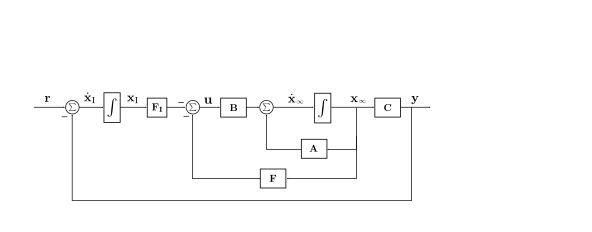
\includegraphics[width=0.6\textwidth]{figures/HinfControlBlockDiagram}
    \caption{Final block diagram of the $\mathcal{H}_\infty$ controller design.}
    \label{fig:HinfControlBlockDiagram}
\end{figure}

The value of $\gamma$ in the Riccatti equation is also a design parameter that can be modified making the controller more or less conservative. The value chosen should be bigger than the largest singular value of the system. In this design, the minimum possible $\gamma$ value is 2.7832. The final value is chosen higher than the minimum in order to have a robustness margin. The value used is 5. 

The final values for the feedback gains result as follows
\begin{flalign}
    \vec{F} &= 
    \begin{bmatrix}
        2233.8 & 1514.2 & 1001.3 \\
        -2233.8 & -1514.2 & 1001.3
    \end{bmatrix} \ , \\
    \vec{F}_\mathrm{I} &=
    \begin{bmatrix}
        -1150.2 & -421.8 \\
        1150.2 & -421.8
    \end{bmatrix} \ .
\end{flalign}

Once the controller is designed, its performance is evaluated in simulations, in which the compensator controls the model derived in \autoref{chap:model}. 

    %\subsection{Controller Performance}
The performance of the controller can be tested as in the case of the linear quadratic regulator through simulation, and the result can be seen in \autoref{fig:xbdot_rob} and \ref{fig:yaw_rob}.
%
\begin{figure}[H]
    \captionbox 
    {   
        Step response of the model with the robust controller in $\dot{x}_\mathrm{b}$.
        \label{fig:xbdot_rob}
    }                                                                 
    {                                                                  
        \includegraphics[width=.45\textwidth]{figures/xbdot_rob}         
    }                                                                    
    \hspace{5pt}                                                          
    \captionbox  
    {      
        Step response of the model with the robust controller in $\psi$ at 10 s.
        \label{fig:yaw_rob}
    }                                                                          
    {
        \includegraphics[width=.45\textwidth]{figures/yaw_rob}
    }
\end{figure}
%
\autoref{fig:xbdot_rob} shows the step response of $\dot{x}_\mathrm{b}$, when a reference of 1 m s$^{-1}$ is set. In this case, the settling time is around \num{1.4} s and there is no overshoot.

The response in $\psi$, \autoref{fig:yaw_rob}, shows a settling time of \num{2.6} s and no overshoot.



\fxnote{Check seconds and settling times with final graphs in robust simulations.}
    \section{Comparison between Controller Designs}\label{sec:comparison}
The two controller designs are now compared in order to analyze the robustness, the performance. The control inputs applied by each controller are also compared. The simulations carried out in this section include input disturbances, both from wind and waves, and measurement noise in the outputs. Model perturbations are also included.

The performance comparison is evaluated looking at the response of the nonlinear model of the system when tracking a step in the reference inputs, $\dot{x}_\mathrm{b,ref}$ and $\psi_\mathrm{ref}$. 

The disturbances applied to the system range from \fxnote{write range of forces along x} in the force along the $\dot{x}_\mathrm{b}$ and \fxnote{write range of taus}. These disturbances come from wind and waves. The frequency of the latter is also varied from \fxnote{write range of frequencies}. The noise applied in all simulations is of \fxnote{write amount of noise}. 

The parameter uncertainties are varied $\pm$20\% \fxnote{check percentage} from their nominal value. The parameters varied in the simulation are the added mass, $m_\mathrm{x}$, the moment of inertia around the $z_\mathrm{b}$ axis, $I_\mathrm{z}$, the damping coefficients, $d_\mathrm{x}$ and $d_\psi$, and the lengths where the forces are applied, $l_1$ and $l_2$. 

\autoref{fig:xbdot_mc_lqr} and \ref{fig:xbdot_mc_rob} show the step response of the velocity along the $x_\mathrm{b}$ direction from \fxnote{number of simulations} simulations where the model parameters and the disturbances were varied randomly within the defined ranges. These simulations also include a reference step in $\psi$ at 10 seconds that causes a perturbation in the $\dot{x}_\mathrm{b}$ response.
\begin{figure}[H]
    \captionbox 
    {   
        \label{fig:xbdot_mc_lqr}
    }                                                                 
    {                                                                  
        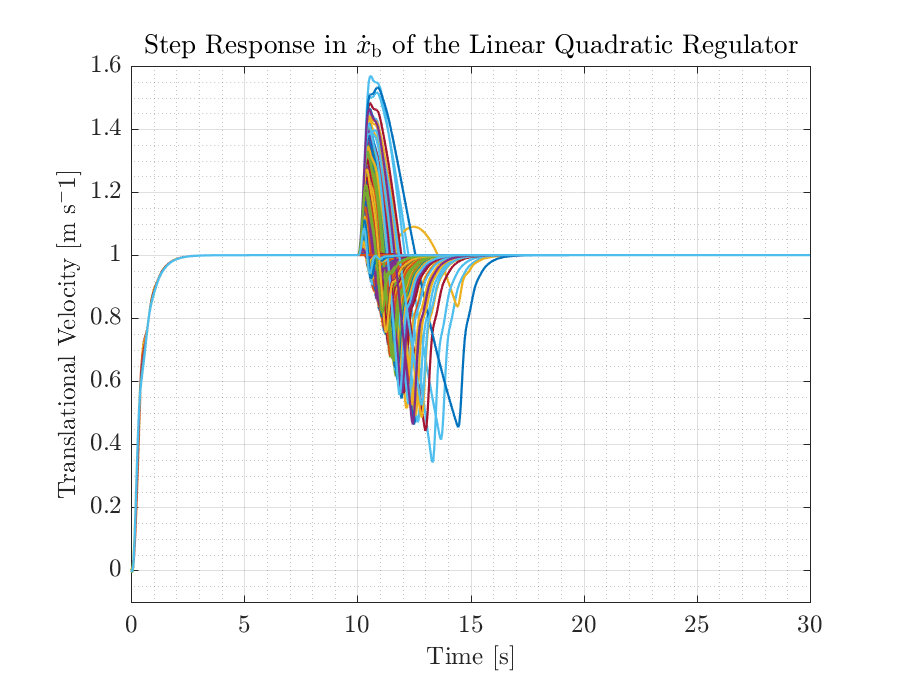
\includegraphics[width=.45\textwidth]{figures/xbdot_mc_lqr}         
    }                                                                    
    \hspace{5pt}                                                          
    \captionbox  
    {      
        \label{fig:xbdot_mc_rob}
    }                                                                          
    {
        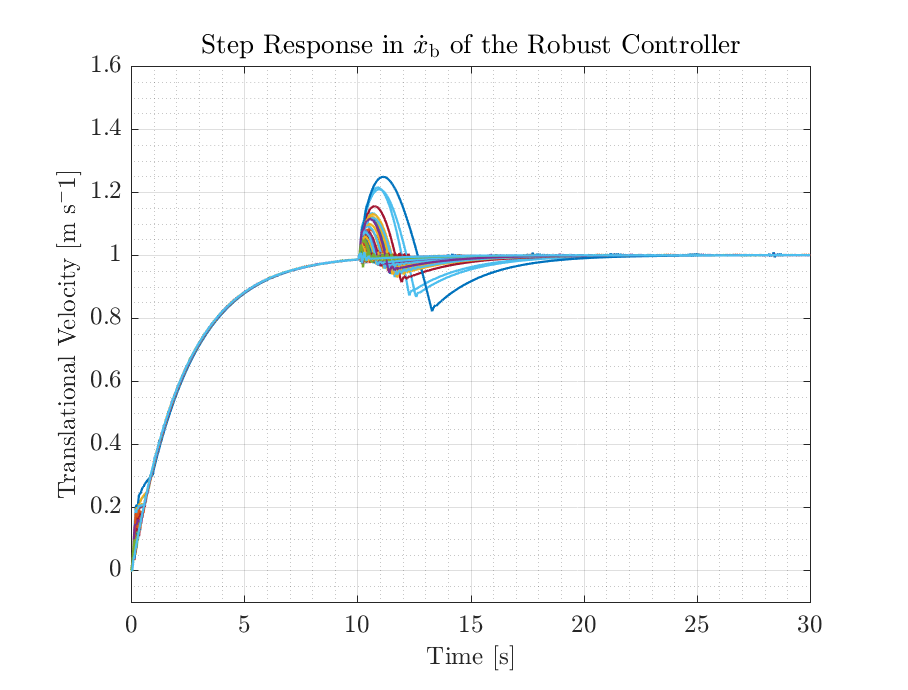
\includegraphics[width=.45\textwidth]{figures/xbdot_mc_rob}
    }
\end{figure}
As it can be seen, both controllers are able to track the given reference in $\dot{x}_\mathrm{b}$. The controller designed using LQR theory yields a fast controller, but the change in reference in the $\psi$ angle leads to a great perturbation in the vessel speed, reaching \fxnote{write value} m/s. There is no steady state error once the disturbance has been compensated by the controller. The $\mathcal{H}_\infty$ controller on the other hand, is much slower in terms of settling time, the perturbation introduced when changing $\psi_\mathrm{ref}$ is \fxnote{write value} m/s. 

It is also remarkable to see how the robust control design presents its biggest perturbations only in few simulations, while the LQR controller shows perturbations greater than 20 \% of the final value in a greater amount of simulations.

These aspects are also seen when comparing the variance of the step response with respect to the performance of the controllers without disturbances or parameter uncertainties. The variance obtained by the LQR controller is \fxnote{write variance for LQR} and that for the $\mathcal{H}_\infty$ controller is \fxnote{write variance for robust}.

In \autoref{fig:yaw_mc_lqr} and \ref{fig:yaw_mc_rob}, the performance of the controllers in analyzed by looking at the step response when tracking a reference in $\psi$. These plots are part of the same simulations depicted in \autoref{fig:xbdot_mc_lqr} and \ref{fig:xbdot_mc_rob}, and therefore cope with the same disturbances and parameter variations. The step is applied after 10 seconds of simulation.
\begin{figure}[H]
    \captionbox 
    {   
        \label{fig:yaw_mc_lqr}
    }                                                                 
    {                                                                  
        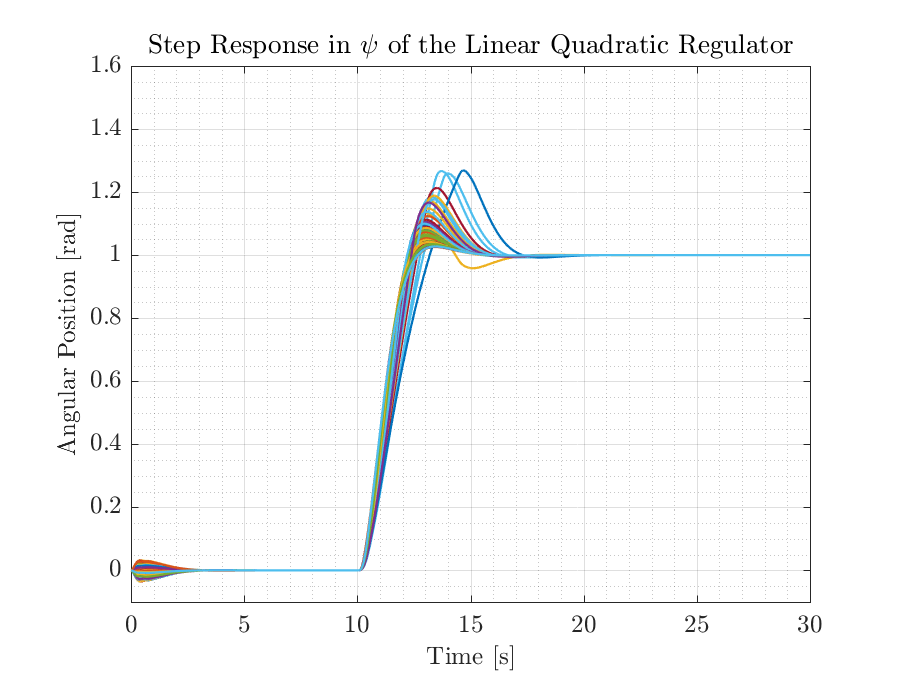
\includegraphics[width=.45\textwidth]{figures/yaw_mc_lqr}         
    }                                                                    
    \hspace{5pt}                                                          
    \captionbox  
    {      
        \label{fig:yaw_mc_rob}
    }                                                                          
    {
        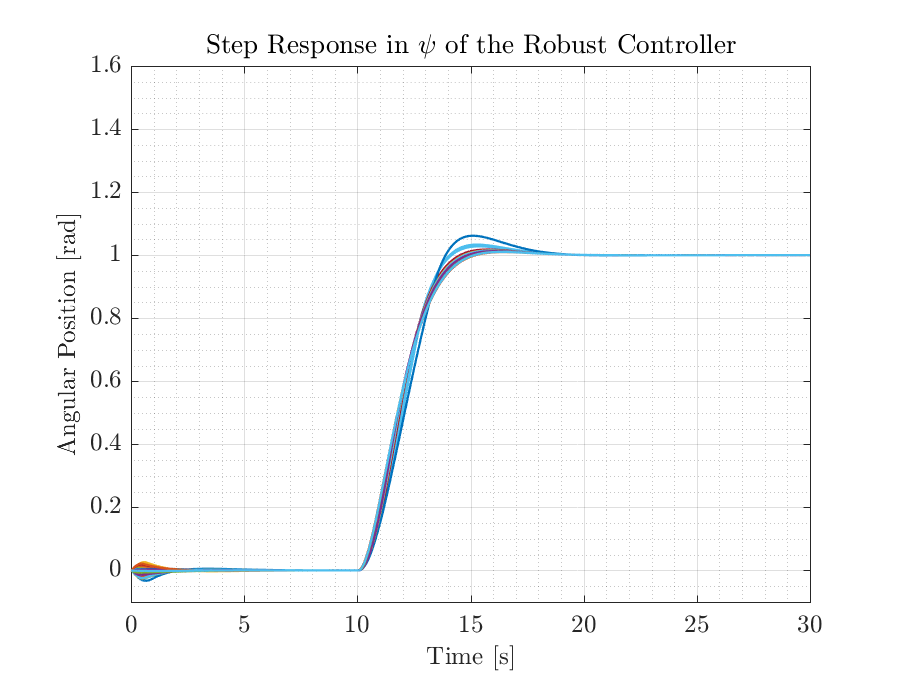
\includegraphics[width=.45\textwidth]{figures/yaw_mc_rob}
    }
\end{figure}
The behavior seen in these figures resembles that for \autoref{fig:xbdot_mc_lqr} and \ref{fig:xbdot_mc_rob}. The $\mathcal{H}_\infty$ controller shows less overshoot and variability in the different simulations but it is also slightly slower that the LQR controller. In both case, the step  In order to achieve a proper comparison, the variance with respect to the nominal model respons in abscense of disturbances has been calculated. For the LQR controller, the variance is \fxnote{Write variance for LQR}, while that for the $\mathcal{H}_\infty$ controller is \fxnote{write variance for robust}.

These controller designs are also compared by their usage of inputs. The mean force applied at each time by the thrusters when simulating the LQR controller is \num{21.5098} N, while that of the $\mathcal{H}_\infty$ controller is \num{21.8321} N. It is clear that the \fxnote{LQR/ROBUST} controller uses less force to track the reference. This correlates with the settling times seen for each controller, as the LQR showed a faster step response compared to the $\mathcal{H}_\infty$ controller. 

Finally, to combine performance and usage of inputs, the cost used in the LQR design is calculated as 
%
\begin{flalign}
J = \sum_{k=0}^\infty \vec{x}_k^\mathrm{T}\vec{Q}\vec{x}_k + \vec{u}_k^\mathrm{T}\vec{R}\vec{u}_k  \ \ .
\end{flalign}

The mean cost among the simulations is \num{7.1378}$\cdot 10^5$ and \num{3.4203}$\cdot 10^6$ for the LRQ and $\mathcal{H}_\infty$ controller designs. As expected, the cost is lower for the LQR design as minimizing it is the basis of the LQR approach.




    
    %---------- Chapter 8 ---------------------------------------- Path Following
    \chapter{Outer Controller Design}\label{chap:outerController}
fThe vessel functionality, as stated in \autoref{sec:requirements}, requires it to follow a path along which the bathymetric measurements are taken. The path is generated from the given area in straight lines as described in \autoref{sec:pathgeneration}.  The generated path is followed by using an enclosure based steering algorithm \cite[pp. 258-265]{TFossen} that uses waypoints sampled along the path. The outputs for this controller are the reference for the yaw angle and the velocity along the $x_\mathrm{b}$ axis, which are inputs to the state space controller designed in \autoref{chap:innercontrol}.
    \section{Path Generation Algorithm}\label{sec:pathgeneration}

\fxnote{Check if all variables are correct}The path generation algorithm creates a list of waypoints for the vessel to follow. The area that needs to be surveyed is used to generate the waypoints. The desired area is a bounded rectangle and is given as an input to the algorithm as four coordinates, in \autoref{eq:pathgenxy}, that specifies the start and end coordinates of the area.
%
\begin{flalign} 
  \{x_1; y_1\},       \rule{15px}{0px} 
  \{x_2; y_2\},       \rule{15px}{0px}
  \{x_3; y_3\},       \rule{15px}{0px} 
  \{x_4; y_4\}.       \rule{15px}{0px} 
  \label{eq:pathgenxy}
\end{flalign}
%
\begin{where}
  \va{\{x_k; y_k\}}{is the coordinate of the corner of the bounded rectangle}{}
\end{where}

The path generation algorithm is confined to generate waypoints in an area that is a rectangle. Thus, the four input coordinates need to be verified to ensure the area is a rectangle. This is done by checking
\begin{flalign} 
  \sqrt{(x_1 - x_2)^2 + (y_1 - y_2)^2} &= \sqrt{(x_3 - x_4)^2 + (y_3 - y_4)^2} \\
  \sqrt{(x_1 - x_4)^2 + (y_1 - y_4)^2} &= \sqrt{(x_2 - x_3)^2 + (y_2 - y_3)^2} \\
%   \label{eq:pathgenlengths}
% \end{flalign}
% \begin{flalign}
  \sin{\frac{y_1 - y_2}{x_1 - x_2}} - \sin{\frac{y_1 - y_4}{x_1 - x_4}}  &= \frac{\pi}{2} 
  \label{eq:pathgen}
\end{flalign}
%
Now that the desired area is well defined, as a rectangle, the path generation algorithm is able to generate a list of waypoints for the USV to follow in the given area. \\The path is generated with straight lines and turns for which the vessel shall follow. This pattern is chosen as bathymetric measurements are typically performed in straight lines \fxnote{source}.To determine the width between these lines, the dynamics of the vessel, the swath angle of the multibeam echosounder and the minimum depth of the area to survey were taken into consideration. The swath angle and minimum depth of the Port of Aalborg survey in \autoref{app:bathymetricMapPortOfAalborg} were used to calculate the width between straight lines, as described in \autoref{sec:designconsiderations},
%
\begin{flalign}
  w_\mathrm{beam} = 36\ \mathrm{m}
\end{flalign}
\begin{where}
  \va{w_\mathrm{beam}}{is the minimum required beamwidth}{m}
\end{where}

The dynamics of the vessel also needs to be considered to ensure the vessel can perform smooth turns between straight lines. It is determined that the vessel capable of using the turning radius 
%
\begin{flalign}
  R_\mathrm{turn} = \frac{1}{2} w_\mathrm{beam} = 18\ \mathrm{m}
\end{flalign}
\begin{where}
  \va{R_\mathrm{turn}}{is the turning radius of the waypoints}{m}
\end{where}

The path generation algorithm first determines whether to generate waypoints along the x axis or the y axis. This is done to ensure the vessel will perform the least number of turns and is determined by calculating whether the x or y distance is greater. This is done by checking if
%
\begin{flalign}
	(x_\mathrm{end}-x_\mathrm{start}) \geq (y_\mathrm{end}-y_\mathrm{start})
\end{flalign}
%
Once the sailing direction is chosen, the first waypoint is generated using the starting point's coordinates and the direction of the straight lines. The starting point in the transversal direction is offset by $R_\mathrm{turn}$ so the multibeam is able to survey the from the edges of the area.

The number of waypoints on both the straight lines and on the turns are generated using
%
\begin{flalign}
  d_\mathrm{wps} = 50 \mathrm{m} \\
  n_\mathrm{wps} = 10
\end{flalign}
\begin{where}
  \va{d_\mathrm{wps}}{is the distance between waypoints on the straight line}{}
  \va{n_\mathrm{wps}}{is the number of waypoints on each turn}{}
\end{where}

As the area to survey may vary, the waypoints are generated every $d_\mathrm{wps}$ meters to ensure the boat will follow the designated path using these waypoints. Thus, the boat will not rely only on the waypoints that define the area. The path for turns is fixed $R_\mathrm{turn}$ therefore the number of waypoints are fixed to $n_\mathrm{wps}$.

In \autoref{fig:pathgen1} an example of the desired area to survey and the generated waypoints is shown. It can be seen that the vessel is offset by $R_\mathrm{turn}$ and the minimum area the  multibeam sensor surveys is also shown.
%
\begin{figure}[H]
  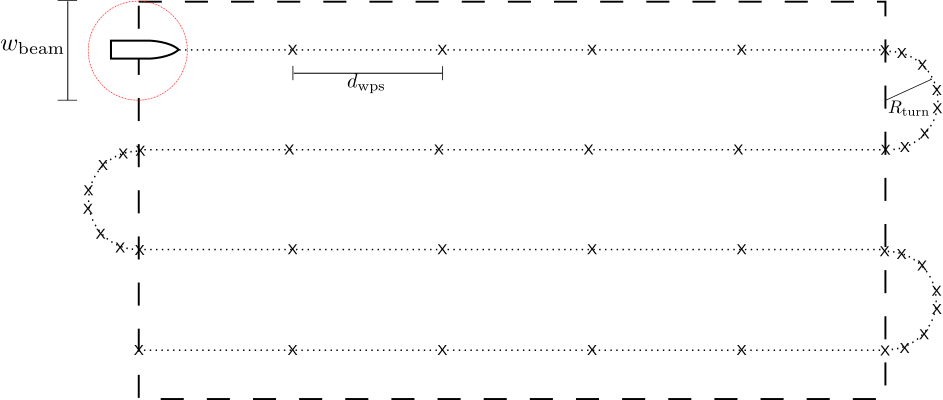
\includegraphics[width=1\textwidth]{figures/pathGen} 
  \caption{Area wanted to survey with waypoints}
  \label{fig:pathgen1}
\end{figure}   



    \section{Path Following Algorithm}\label{sec:pathfollower}
The path generated is approximated by straight line segments connected by the calculated waypoints. The vessel then follows these in order to track the path and cover the area in which the measurements are to be taken. This approximation is suitable as the bathymetric measurements are usually taken in straight line paths. Straight line segments on the curved paths are not required as the curved paths are outside of the area of interest. If curved paths were required, the solution would be to sample the path with higher frequency in curved sections. \autoref{fig:pathandwaypoints} shows an example of how a path is approximated by straight line segments and waypoints.
\begin{figure}[H]
	\includegraphics[width=0.6\textwidth]{figures/pathandwpts}
	\caption{A predefined path and its approximation as straight line segments using waypoints.}
	\label{fig:pathandwaypoints}
\end{figure}
The algorithm starts by considering the first two waypoints in the path. The yaw reference given to the state space controller is calculated based on the crossing point between the straight line segment that joints the waypoints and a circle centered in the position of the boat. \autoref{fig:LOSalgorithm} shows how this crossing point is obtained. The crossing point is also called LOS (Line Of Sight) point and is found using the equations of the circle and of the straight line as
%
\begin{flalign}
	(&x_\mathrm{los}-x_\mathrm{n})^2 + (y_\mathrm{los}-y_\mathrm{n})^2 = R^2, \label{eq:circle} \ \\
	&y_\mathrm{los}-y_\mathrm{k} = \frac{y_\mathrm{k+1}-y_\mathrm{k}}{x_\mathrm{k+1}-x_\mathrm{k}}(x_\mathrm{los}-x_\mathrm{k}) \label{eq:line} 
\end{flalign}
\begin{where}
	\va{R}{is the radius of the circle centered at the vessel position}{}
	\va{[x_\mathrm{los},y_\mathrm{los}]}{is the crossing point between the circle around the vessel and the straight line that joins the waypoints}{}
	\va{[x_\mathrm{k},y_\mathrm{k}]}{is the first waypoint in the currently followed path segment}{}
	\va{[x_\mathrm{k+1},y_\mathrm{k+1}]}{is the second waypoint in the currently followed path segment}{}
	\va{[x_\mathrm{n},y_\mathrm{n}]}{is the position of the vessel in the NED frame}{}
\end{where}
%
\begin{figure}[H]
	\includegraphics[width=0.5\textwidth]{figures/LOSalgorithm}
	\caption{Algorithm used to find the yaw reference for the state space controller in order to follow a path.}
	\label{fig:LOSalgorithm}
\end{figure}
The LOS point is then used to calculate $\chi$ as the angle from the $x_\mathrm{n}$ axis and the line joining the position of the vessel and the LOS point. See \eqref{eq:chi}. This can be directly used as the reference for yaw, $\psi_\mathrm{ref}$, in the state space controller. This disregards the possibility of disturbances and assumes that the velocity vector of the vessel is aligned with the $x_\mathrm{b}$ axis. This is in general not true as disturbances like wind or waves would generate some speed also in the $y_\mathrm{b}$ axis direction. The reference for yaw is then adjusted by subtracting the angle that the velocity vector has with respect to the $x_\mathrm{b}$ axis as seen in \eqref{eq:beta} and \eqref{eq:psiref}. 

This approach tries to make the vessel velocity vector point towards the LOS point.
%
\begin{flalign}
	\chi &= \arctan\left(\frac{y_\mathrm{los}-y_\mathrm{n}}{x_\mathrm{los}-x_\mathrm{n}}\right), \label{eq:chi} \ \\
	\beta &= \arctan\left(\frac{\dot{y}_\mathrm{b}}{\dot{x}_\mathrm{b}}\right) \label{eq:beta}, \ \\
	\psi&_\mathrm{ref} = \chi - \beta. \label{eq:psiref}
\end{flalign}
\begin{where}
	\va{\chi}{is the angle between the $x_\mathrm{n}$ axis and the LOS point}{}
	\va{\beta}{is the angle between the velocity vector of the vessel and the $x_\mathrm{b}$ axis}{}
\end{where}
%
The algorithm relies on the path and the circle defined around the boat to cross at the LOS point. 

If the vessel is positioned far from the path such that the circle does not intersect it, then the algorithm uses the next waypoint as LOS point. Once the vessel gets closer to the path, the LOS point is calculated as described above.

The yaw reference, $\psi_\mathrm{ref}$, given to the controller in \ref{innercontrol} ensures that the vessel will follow the desired LOS.

In order to follow all the path, a way to change which two waypoints define the current path segment needs to be established. Several possibilities can be considered but all of them change active waypoints when the vessel gets close enough to the waypoint that defines the end of the segment. In the project at hand, the distance to the waypoint is evaluated as the distance from the waypoint to the intersection point of the path segment and a perpendicular line to the segment that passes through the vessel position. This distance is depicted in \autoref{fig:changewaypoints}.
\begin{figure}[H]
	\includegraphics[width=0.6\textwidth]{figures/LOSalgorithmdistancewp}
	\caption{The distance considered when defining the criterion to change to new waypoints.}
	\label{fig:changewaypoints}
\end{figure}
With this approach, the vessel will always try to move forward in the path although a waypoint position has not been precisely attained. % This avoids situations like the one shown in \autoref{fig:goingbackapproach} where the vessel turns around in order to hit the waypoint precisely.
This could be caused by a sudden disturbance experienced by the vessel and, in general, it is desired to keep following the path rather than turning around to hit the waypoint. In most cases, the vessel itself is going to be close to the waypoint when the change occurs. This can be seen in the simulation plots presented below. 

\subsection{Path Following Algorithm Simulation}

\fxnote{Do not include many graphs now because we will probably redo them. Just some dummy ones.} 
\fxnote{Maybe we could include the result also with different low level controllers}
The path following algorithm has been tested in the same path and considering different settings for the algorithm. In all cases, the radius of the circle defined around the vessel is 5 m and the distance in which the active waypoints are changed is 3 m. 

In \autoref{fig:simpleLOSalgorithm} and \ref{fig:simpleLOSalgorithmdisturbance} the results of the algorithm are presented when considering the simpler case in which $\psi_\mathrm{ref} = \chi$, that is, assuming the velocity of the vessel is pointing along the $x_\mathrm{b}$ direction. In the first graph the path is followed precisely as the assumption regarding the velocity vector holds,  whereas in the second, the constant disturbance imposes an offset in the position of the vessel.
\begin{figure}[H]
	\captionbox  %<--use captionbox instead if no global caption is needed
	{               %                                \%-%-%-%-%-%-%\
	 	Performance of the path following algorithm based on $\psi_\mathrm{ref}=\chi$.                %\
		\label{fig:simpleLOSalgorithm}                                  %\
	}                                                                 %\
	{                                                                  %\
		\includegraphics[width=.45\textwidth]{figures/pathfollowingsimple}         %\
	}                                                                    %\
	\hspace{5pt}                                                          %\
	\captionbox  %<-----------------------------------------------------%\
	{       
		Performance of the path following algorithm based on $\psi_\mathrm{ref}=\chi$. The vessel is experiencing a constant disturbance force of 1 N applied with an angle of $\pi/2$.                                                                  %\                         %\
		\label{fig:simpleLOSalgorithmdisturbance}                                     %\
	}                                                                           %\
	{                                                                            %\
		\includegraphics[width=.45\textwidth]{figures/pathfollowingsimpledist}            %|
	}                                                                             %|
\end{figure}
When the information of the vessel velocity is used to calculate the reference angle, $\psi_\mathrm{ref}$, the disturbance is rejected. This is seen in \autoref{fig:normalLOSalgorithmdisturbance}, where the vessel is experiencing the same disturbance as in \autoref{fig:simpleLOSalgorithmdisturbance}. In this case, the offset in position has been corrected and the path is precisely followed.
\begin{figure}[H]
	\includegraphics[width=0.5\textwidth]{figures/pathfollowingcomplex}
	\caption{Performance of the path following algorithm based on $\psi_\mathrm{ref}=\chi-\beta$. The vessel is experiencing a constant disturbance force of 1 N applied with an angle of $\pi/2$.}
	\label{fig:normalLOSalgorithmdisturbance}
\end{figure}
According to the results of the simulations, it can be said that the vessel hits the waypoints precisely when they are part of a straight line section of the path. In curved sections, the vessel joins smoothly the straight line segments that approximate the curve. In many cases, and especially for bathymetric measurements the algorithm can be considered suitable.

	




    \section{Simulations}\label{sec:pathSim}
The path following algorithm is tested in the same path and considering different settings for the algorithm. In all cases, the distance in which the active waypoints are changed is \num{1} m. For seeing the results, the model of the system has been simulated with the path following algorithm and the two inner controller designs. In the plots presented, the data from 100 simulations is depicted, where the disturbances, model uncertainties and noise affect the system.

The wind and current disturbance varies randomly from $\pm$\num{1.5} N in force along $x_\mathrm{b}$ and so does along $y_\mathrm{b}$, and from $\pm$\num{1.5} N$\cdot$m in torque in $\psi$. The waves are assumed to be sinusoidal with amplitude of 1 N and a frequency that goes from 0 to 10 Hz. This disturbance is applied along $x_\mathrm{b}$ and $y_\mathrm{b}$. 

The uncertainty considered is of 20\% in all parameters of the model, that is, the mass, $m$, the moment of inertia around the $z_\mathrm{b}$ axis, $I_\mathrm{z}$, the damping coefficients, $d_\mathrm{x}$, $d_\mathrm{y}$ and $d_\psi$, and the vessel lengths, $l_1$ and $l_2$.  

In \autoref{fig:lqrwrong}, \ref{fig:distlqrwrong}, \ref{fig:robwrong} and \ref{fig:distrobwrong} the results of the algorithm are presented by depicting the path taken by the vessel and the distance to the target path. In these figures, the path following algorithm corresponds to the simpler case in which $\psi_\mathrm{ref} = \chi$, that is, assuming the velocity of the vessel is pointing along the $x_\mathrm{b}$ direction. The simulations are performed with both inner controller designs. 

\begin{figure}[H]
	\captionbox  %<--use captionbox instead if no global caption is needed
	{  
		Performance of the path following algorithm based on $\psi_\mathrm{ref}=\chi$ and using the LQR inner controller. The reference for velocity is set to \num{0.4} m$\cdot$s$^{-1}$. and the system is experiencing wind, current and wave disturbances, model perturbations and measurement noise. \label{fig:lqrwrong}                                
	}                                                                 
	{                                                                  
		\includegraphics[width=.45\textwidth]{figures/path_lqr_no_correc}         
	}                                                                    
	\hspace{5pt}                                                  
	\captionbox
	{       
		Distance to the path when using the algorithm based on $\psi_\mathrm{ref}=\chi$ and the LQR inner controller.
		\label{fig:distlqrwrong}                               
	}                                                                  
	{                                                                    
		\includegraphics[width=.45\textwidth]{figures/dist_lqr_no_correc}         
	}                                                                         
\end{figure}
\begin{figure}[H]
	\captionbox 
	{   
		Performance of the path following algorithm based on $\psi_\mathrm{ref}=\chi$ and using the $\mathcal{H}_\infty$ inner controller. The reference for velocity is set to \num{0.4} m$\cdot$s$^{-1}$. and the system is experiencing wind, current and wave disturbances, model perturbations and measurement noise. \label{fig:robwrong}      
	}                                                                 
	{                                                                  
		\includegraphics[width=.45\textwidth]{figures/path_rob_no_correc}         
	}                                                                    
	\hspace{5pt}                                                          
	\captionbox  
	{      
		Distance to the path when using the algorithm based on $\psi_\mathrm{ref}=\chi$ and the $\mathcal{H}_\infty$ inner controller.\label{fig:distrobwrong}
	}                                                                          
	{
		\includegraphics[width=.45\textwidth]{figures/dist_rob_no_correc}
	}
\end{figure}

In these graphs, it is clear that the path is not precisely followed when disturbances are introduced in the system. This offset is expected as the assumption for this simpler algorithm to work does not hold with disturbances like wind, current and waves. The latter is specially visible in the straight line parts of the path, where the vessel movement shows a 1$\sigma$ value that goes up to 10 cm and a maximum value that reaches up to approximately 30 cm.

When the information of the vessel velocity is used to calculate the reference angle, $\psi_\mathrm{ref}$, the disturbance is rejected. This is seen in \autoref{fig:lrqcorrect}, \ref{fig:distlqr}, \ref{fig:robustcorrect} and \ref{fig:distrobustcorrect}, where the vessel is experiencing disturbances and model perturbations in the same range as in the previously shown figures. Both the vessel X-Y movement and the distance to the target path are depicted. 

\begin{figure}[H]
	\captionbox 
	{            
		Performance of the path following algorithm based on $\psi_\mathrm{ref}=\chi-\beta$ and using the LQR inner controller.The reference for velocity is set to \num{0.4} ms$^{-1}$. and the system is experiencing wind, current and wave disturbances, model perturbations and measurement noise.                
		\label{fig:lrqcorrect}                                  
	}                                                                 
	{                                                                  
		\includegraphics[width=.45\textwidth]{figures/path_lqr}         
	}                                                                    
	\hspace{5pt}                                                          
	\captionbox 
	{       
		Distance to the path when using the algorithm based on $\psi_\mathrm{ref}=\chi-\beta$ and the LQR inner controller. \label{fig:distlqr}                                   
	}                                                     
	{                                                                        
		\includegraphics[width=.45\textwidth]{figures/dist_lqr}            
	}                                                                            
\end{figure}
\begin{figure}[H]
	\captionbox 
	{   
		Performance of the path following algorithm based on $\psi_\mathrm{ref}=\chi-\beta$ and using the $\mathcal{H}_\infty$ inner controller. The system is experiencing wind, current and wave disturbances, model perturbations and measurement noise. \label{fig:robustcorrect}
	}                                                                 
	{                                                                  
		\includegraphics[width=.45\textwidth]{figures/path_rob}         
	}                                                                    
	\hspace{5pt}                                                          
	\captionbox  
	{      
			Distance to the path when using the algorithm based on $\psi_\mathrm{ref}=\chi-\beta$ and the $\mathcal{H}_\infty$ inner controller. \label{fig:distrobustcorrect}
	}                                                                          
	{
		\includegraphics[width=.45\textwidth]{figures/dist_rob}
	}
\end{figure}

In this case, the offset in position is corrected and the path is followed within the desired precision in the straight line segments. There are still some small deviations due to the wave disturbance present in the system, but the 1$\sigma$ value is under 5 cm and the maximum variations stay below 10 cm with respect to the reference path.

When comparing the two inner controllers, different behaviors are seen. In the turns, the variations experienced by the LQR are larger than those seen with the $\mathcal{H}_\infty$ controller. This is expected as it is consistent with the response seen in the step responses presented in \autoref{sec:comparison}, where a higher deviations appeared in the LQR when the references were applied to the system. 

In the straight line segments, the behavior is the opposite, the LQR shows a smaller maximum and 1$\sigma$ error than those shown by the $\mathcal{H}_\infty$ controller. This is due to the speed of the controller in terms of settling time, the faster response of the LQR makes it able of correcting the constant wind disturbances and low frequency wave disturbances slightly better, making the error lower by approximately 4 cm.
    
    %---------- Chapter 9 ---------------------------------------- Sensor Fusion
    \chapter{Sensor Fusion}\label{chap:sensorFusion}



    \section{Attitude Estimation}\label{sec:attFusion}
The attitude estimation is done using a Kalman filter. The estimate contains attitude, angular velocity and angular acceleration information. For constructing the Kalman filter, a process model and a measurement model need to be created. 

The process model describes the dynamics of the system and how the inputs affect its states. The process model includes also noise, which is assumed to be normally distributed.
The measurement model describes how the measurements taken from the IMU relate with the states of the system represented in the process model. Measurement noise is also included in the model. The process and measurement models are 
%
\begin{flalign}
    \vec{x}_\mathrm{att}(k+1) &= \vec{A}_\mathrm{att}\vec{x}_\mathrm{att}(k) + \vec{B}_\mathrm{att} \vec{u}(k) + \vec{w}_\mathrm{att}(k) \label{eq:processmodelatt} \\
    \vec{y}_\mathrm{att}(k) &= \vec{C}_\mathrm{att} \vec{x}_\mathrm{att}(k) + \vec{v}_\mathrm{att}(k) \label{eq:measurementmodelatt}\ .
\end{flalign}
\begin{where}
	\va{\vec{x}_\mathrm{att}}{is the system state vector for the attitude Kalman filter}{}
	\va{\vec{u}}{is the input vector}{}
	\va{\vec{w}_\mathrm{att}}{is the process noise vector}{}
    \va{\vec{v}_\mathrm{att}}{is the measurement noise vector}{}
    \va{\vec{A}_\mathrm{att}}{is the system matrix for the attitude Kalman filter model}{}
    \va{\vec{B}_\mathrm{att}}{is the input matrix for the attitude Kalman filter model}{}
    \va{\vec{C}_\mathrm{att}}{is the output matrix for the attitude Kalman filter model}{}    
\end{where}

The noise vectors $\vec{w}_\mathrm{att}$ and $\vec{v}_\mathrm{att}$ are independent, and follow a zero mean normal distribution. The covariance matrices of each distribution are $\vec{Q}_\mathrm{att}$ and $\vec{R}_\mathrm{att}$, respectively. These are diagonal matrices calculated as
\begin{flalign}
	\vec{Q}_\mathrm{att} &= \mathrm{diag}\left( \sigma_\mathrm{\phi}^2,\sigma_\mathrm{\theta}^2,\sigma_\mathrm{\psi}^2,\sigma_\mathrm{\dot{\phi}}^2,\sigma_\mathrm{\dot{\theta}}^2,\sigma_\mathrm{\dot{\psi}}^2,\sigma_\mathrm{\ddot{\phi}}^2,\sigma_\mathrm{\ddot{\theta}}^2,\sigma_\mathrm{\ddot{\psi}}^2 \right) \\
	\vec{R}_\mathrm{att} &= \mathrm{diag} \left( \sigma_{\phi\mathrm{,acc}}^2,\sigma_{\theta\mathrm{,acc}}^2,\sigma_{\psi\mathrm{,mag}}^2,\sigma_{\dot{\phi}\mathrm{,gyro}}^2,\sigma_{\dot{\theta}\mathrm{,gyro}}^2,\sigma_{\dot{\psi}\mathrm{,gyro}}^2 \right)
\end{flalign}

The states variances can be seen in \fxnote{Refer to state variances appendix}, and the measurements variances in \autoref{app:IMUVariances}.

The states chosen for the Kalman model include all variables to be estimated and those in which dynamics of the system play a role. These are
\begin{flalign}
    \vec{x}_\mathrm{att} &= 
    \begin{bmatrix}
       \phi & \theta & \psi & \dot{\phi} & \dot{\theta} & \dot{\psi} & \ddot{\phi} & \ddot{\theta} & \ddot{\psi} \nonumber
    \end{bmatrix}^\mathrm{T} \ .
\end{flalign}
%
Even though the inner state space controller only considers $\psi$ and $\dot{\psi}$, the other Euler angles and angular velocities are included to allow a better overall estimation, specially when using later the rotation matrix elements as described in \autoref{sec:posFusion}. The angular accelerations are normally not part of a state vector in a state space representation. However, in the attitude Kalman filter state vector, the accelerations are included as they are an important part of the dynamics of the vessel as it can be seen in the last tree rows in $A_\mathrm{att}$, \autoref{eq:Aatt}.

The output vector elements depend on the measurements given by the IMU. These include the angular velocities provided by the gyroscope and the attitude measurements. The latter are obtained from a direct calculation using the accelerometer data to compute $\phi_\mathrm{acc}$ and $\theta_\mathrm{acc}$ and the magnetometer data projected on to the plane to compute $\psi_\mathrm{mag}$ \cite{MBibuli}, as	
\begin{flalign}
	\phi_\mathrm{acc} &= - \arctan\left(\frac{\ddot{y}_\mathrm{b,acc}}{\sqrt{\ddot{x}_\mathrm{b,acc}^2 + \ddot{z}_\mathrm{b,acc}^2}} \right)\ , \label{eq:roll_acc} \\
	\theta_\mathrm{acc} &= - \arctan \left( \frac{\ddot{x}_\mathrm{b,acc}}{\sqrt{\ddot{y}_\mathrm{b,acc}^2 + \ddot{z}_\mathrm{b,acc}^2}} \right)\ , \label{eq:pitch_acc} \\
	\psi_\mathrm{mag} &= \arctan \left( \frac{M_{y_\mathrm{b}} \cos(\phi) + M_{z_\mathrm{b}} \sin(\phi)}{M_{x_\mathrm{b}} \cos(\theta) + M_{y_\mathrm{b}} \sin(\phi) \sin(\theta) + M_{z_\mathrm{b}} \cos(\phi) \sin(\theta)} \right)\ .\label{eq:yaw_mag}
\end{flalign}
\begin{where}
	\va{\ddot{x}_\mathrm{b,acc}}{is the measured acceleration along the $x_\mathrm{b}$ direction}{}
	\va{\ddot{y}_\mathrm{b,acc}}{is the measured acceleration along the $y_\mathrm{b}$ direction}{}
	\va{\ddot{z}_\mathrm{b,acc}}{is the measured acceleration along the $z_\mathrm{b}$ direction}{}
	\va{M_{x_\mathrm{b}}}{is the magnetic field strength along the $x_\mathrm{b}$ direction}{}
	\va{M_{y_\mathrm{b}}}{is the magnetic field strength along the $y_\mathrm{b}$ direction}{}
	\va{M_{z_\mathrm{b}}}{is the magnetic field strength along the $z_\mathrm{b}$ direction}{}			
\end{where}

Leading to the output vector 
\begin{flalign}
    \vec{y}_\mathrm{att} =
    \begin{bmatrix}
           \phi_\mathrm{acc} & \theta_\mathrm{acc} & \psi_\mathrm{mag} & \dot{\phi}_\mathrm{gyro} & \dot{\theta}_\mathrm{gyro} & \dot{\psi}_\mathrm{gyro}\nonumber 
    \end{bmatrix}^\mathrm{T}\ .
\end{flalign}
%
The input vector, in this case stays the same as in the state space controller design, containing the two forces provided by the thrusters. The input vector is
\begin{flalign}
    \vec{u} &=
    \begin{bmatrix}
        F_1 & F_2  \nonumber 
    \end{bmatrix}^\mathrm{T}\ .
\end{flalign}
%
With this information, the process and measurement model matrices can be built. The $\vec{A}_\mathrm{att}$ matrix is what describes the dynamics of the model. In this system, the attitude is itself plus the discrete integration of the angular velocity over the sampling period. This is represented by the 1 and the $T_\mathrm{s}$ in each of the Euler angle rows. The same dynamics describe the angular velocities. The angular accelerations depend on the angular velocities through the damping coefficients. In order to consider the most recent value of the angular velocities, the three last rows of $\vec{A}_\mathrm{att}$ are just a copy of the three middle rows of $\vec{A}_\mathrm{att}$ multiplied by the corresponding damping coefficient and divided by the matching moment of inertia. The elements on these last rows also include the minus sign coming from the damping. The $\vec{A}_\mathrm{att}$ matrix is 
\begin{flalign}
	\label{eq:Aatt}
    \vec{A}_\mathrm{att} &=
    \begin{bmatrix}
    	1 & 0 & 0 & T_\mathrm{s} & 0 & 0 & 0 & 0 & 0 \\
        0 & 1 & 0 & 0 & T_\mathrm{s} & 0 & 0 & 0 & 0 \\
        0 & 0 & 1 & 0 & 0 & T_\mathrm{s} & 0 & 0 & 0 \\
        0 & 0 & 0 & 1 & 0 & 0 & T_\mathrm{s} & 0 & 0 \\
        0 & 0 & 0 & 0 & 1 & 0 & 0 & T_\mathrm{s} & 0 \\
        0 & 0 & 0 & 0 & 0 & 1 & 0 & 0 & T_\mathrm{s} \\
        0 & 0 & 0 & -\frac{d_\mathrm{\phi}}{I_\mathrm{x}} & 0 & 0 & -T_\mathrm{s}\frac{d_\mathrm{\psi}}{I_\mathrm{x}} & 0 & 0 \\
        0 & 0 & 0 & 0 & -\frac{d_\mathrm{\theta}}{I_\mathrm{y}} & 0 & 0 & -T_\mathrm{s}\frac{d_\mathrm{\theta}}{I_\mathrm{y}} & 0 \\
        0 & 0 & 0 & 0 & 0 & -\frac{d_\mathrm{\psi}}{I_\mathrm{z}} & 0 & 0 & -T_\mathrm{s}\frac{d_\mathrm{\psi}}{I_\mathrm{z}}\  \nonumber
    \end{bmatrix}.
\end{flalign}
%
The matrix $\vec{B}_\mathrm{att}$ is mostly formed by zeros, the only nonzero elements are placed in the last row, indicating how the forces contribute to the angular acceleration in the yaw angle. The $\vec{C}_\mathrm{att}$ matrix is also straightforward to obtain as the measurement are just the first six states in $\vec{x}_\mathrm{att}$. The $\vec{B}_\mathrm{att}$ and $\vec{C}_\mathrm{att}$ matrices are

\begin{minipage}{0.3\linewidth}
    \begin{flalign}
        \vec{B}_\mathrm{att} &=
        \begin{bmatrix}
            0 & 0 \\
            0 & 0 \\
            0 & 0 \\
            0 & 0 \\
            0 & 0 \\
            0 & 0 \\
            0 & 0 \\
            0 & 0 \\
            \frac{l_1}{I_\mathrm{z}} & -\frac{l_2}{I_\mathrm{z}}\nonumber 
        \end{bmatrix} 
    \end{flalign}
\end{minipage}\hfill
\begin{minipage}{0.6\linewidth}
    \begin{flalign}
        \vec{C} &=
        \begin{bmatrix}
            1 & 0 & 0 & 0 & 0 & 0 & 0 & 0 & 0 \\
            0 & 1 & 0 & 0 & 0 & 0 & 0 & 0 & 0 \\
            0 & 0 & 1 & 0 & 0 & 0 & 0 & 0 & 0 \\
            0 & 0 & 0 & 1 & 0 & 0 & 0 & 0 & 0 \\
            0 & 0 & 0 & 0 & 1 & 0 & 0 & 0 & 0 \\
            0 & 0 & 0 & 0 & 0 & 1 & 0 & 0 & 0 \nonumber 
        \end{bmatrix} 
    \end{flalign}
\end{minipage}\hfill

Once the model is constructed, the Kalman filter equations can be obtained. They are divided in two steps, prediction and update \cite{SHaykin}. To start the process, the estimate and error covariance matrix $\vec{P}_\mathrm{att}$ need to be initialized. The state estimation is initialized with its mean, which is zero and the error covariance matrix is initialized with the covariance matrix for the states. The initialization is done as
\begin{flalign}
	\vec{x}_\mathrm{att}(0|0) &= \vec{0}_\mathrm{1x6}\\
	\vec{P}_\mathrm{att}(0|0) &= \vec{Q}_\mathrm{att}\ .
\end{flalign}
 %
In the prediction step, the sensor most recent measurement has not been acquired yet and the model of the system is used to predict the state values in the next period. The error covariance is also predicted using the system matrix, $\vec{A}_\mathrm{att}$, and the covariance matrix, $\vec{Q}_\mathrm{att}$, of the process noise vector included in the model.
The prediction step of the Kalman filter is  
\begin{flalign}
	\hat{\vec{x}}_\mathrm{att}(k+1|k) &= \vec{A}_\mathrm{att} \hat{\vec{x}}_\mathrm{att}(k|k) + \vec{B}_\mathrm{att} \vec{u}(k) \label{eq:predictxatt} \\
	\vec{P}_\mathrm{att}(k+1|k) &= \vec{A}_\mathrm{att} \vec{P}_\mathrm{att}(k|k) \vec{A}_\mathrm{att}^\mathrm{T} + \vec{Q}_\mathrm{att} \label{eq:predictPatt}
\end{flalign}
%
The update step corrects the estimate using the prediction obtained in the previous step and the innovation \cite[p. 7]{SHaykin}, that is, the error between the new measurement and the predicted new measurement. This error updates $\vec{x}_\mathrm{att}$ weighted by the Kalman gain $\vec{K}(k)$. The update step of the Kalman filter calculates the updated state estimation and the updated error covariance as 
\begin{flalign}
    \hat{\vec{x}}_\mathrm{att}(k+1|k+1) &= \hat{\vec{x}}_\mathrm{att}(k+1|k) + \vec{K}(k+1) \left[ \vec{y}(k+1) - \vec{C}_\mathrm{att}  \hat{\vec{x}}_\mathrm{att}(k+1|k) \right]\ , \label{eq:updatexatt}\\
    \vec{P}_\mathrm{att}(k+1|k+1) &= \left[ \vec{I} - \vec{K}(k+1) \vec{C}_\mathrm{att}^\mathrm{T} \right] \vec{P}_\mathrm{att}(k+1|k)\ . \label{eq:updatePatt}
\end{flalign}
%
Being the Kalman gain 
\begin{flalign}
	\vec{K}(k+1) &= \vec{P}_\mathrm{att}(k+1|k) \vec{C}_\mathrm{att}^\mathrm{T} \left[\vec{C}_\mathrm{att} \vec{P}(k+1|k) \vec{C}_\mathrm{att}^\mathrm{T} + \vec{R}_\mathrm{att} \right]^{-1}\ , \label{eq:kalmangainatt}
\end{flalign}
%
which weights how much the measurements and the prediction affect the estimate of the states. It is calculated using the prediction error covariance matrix, $\vec{P}_\mathrm{att}$, the output matrix, $\vec{C}_\mathrm{att}$, and the covariance matrix for the noise vector included in the measurement model. A more detailed derivation of this gain can be found in \cite[pp. 5-8]{SHaykin}.

    \subsection{Performance of the Filter}
The performance of the Kalman filter is tested through simulations. These are performed by applying some arbitrary inputs to the nonlinear model of the system derived in \autoref{chap:model}. The signals obtained are transformed into measurements by adding noise whose variance are those present in the physical sensors, as seen in \autoref{app:IMUVariances}. \fxnote{write filter parameters used.}

In \autoref{fig:sim_yaw} the estimation of the heading, $\psi$, can be seen.
\begin{figure}[H]
    \includegraphics[width=0.5\textwidth]{figures/sim_yaw}
    \caption{Result of the estimation of the heading, compared to the real value in the simulation and the measurements.}
    \label{fig:sim_yaw}
\end{figure}

The filter is able to remove part of the noise present in the measurements, and gives a better results than the raw measurements.
%
The estimation of the angular velocity and acceleration around $z_\mathrm{b}$ can be seen in \autoref{fig:sim_yawdot} and \ref{fig:sim_yawddot}, respectively. The filter is able to give a correct estimate of the real signals even when there is no measurement, as it is the case for $\ddot{\psi}$.
%
\begin{figure}[H]
    \captionbox 
    {   
        Result of the estimation of the angular velocity around $z_\mathrm{b}$, compared to the real value in the simulation and the measurements.
        \label{fig:sim_yawdot}
    }                                                                 
    {                                                                  
        \includegraphics[width=.45\textwidth]{figures/sim_yawdot}         
    }                                                                    
    \hspace{5pt}                                                          
    \captionbox  
    {      
        Estimation of the angular acceleration around $z_\mathrm{b}$, compared to the real value.
        \label{fig:sim_yawddot}
    }                                                                          
    {
        \includegraphics[width=.45\textwidth]{figures/sim_yawddot}
    }
\end{figure}
%
%\begin{figure}[H]
%    \includegraphics[width=0.5\textwidth]{figures/real_yaw}
%    \caption{}
%    \label{fig:real_yaw}
%\end{figure}
%
%\begin{figure}[H]
%    \captionbox 
%    {   
%        Result of the estimation of the angular velocity around $z_\mathrm{b}$, compared to the measurements.
%        \label{fig:real_yawdot}
%    }                                                                 
%    {                                                                  
%        \includegraphics[width=.45\textwidth]{figures/sim_yawdot}         
%    }                                                                    
%    \hspace{5pt}                                                          
%    \captionbox  
%    {      
%        Estimation of the angular acceleration around $z_\mathrm{b}$.
%        \label{fig:real_yawddot}
%    }                                                                          
%    {
%        \includegraphics[width=.45\textwidth]{figures/real_yawddot}
%    }
%\end{figure}
%
%\cite{MSalari}
    \section{Position Estimation}\label{sec:posFusion}

\begin{flalign}
    \vec{x}_\mathrm{pos}(k+1) &= \vec{A}_\mathrm{pos}(k)\vec{x}_\mathrm{pos}(k) + \vec{B}_\mathrm{pos} \vec{u}(k) + \vec{w}_\mathrm{pos} \\
    \vec{y}_\mathrm{pos}(k) &= \vec{C}_\mathrm{pos} \vec{x}_\mathrm{pos}(k) + \vec{v}_\mathrm{pos}
\end{flalign}

\begin{where}
    \va{\vec{w}_\mathrm{pos}}{}{}
    \va{\vec{v}_\mathrm{pos}}{}{}
\end{where}
%
\begin{minipage}{0.32\linewidth}
    \begin{flalign}
        \vec{x}_\mathrm{pos} &=
        \begin{bmatrix}
            x_\mathrm{n} \\
            y_\mathrm{n} \\
            \dot{x}_\mathrm{b} \\
            \dot{y}_\mathrm{b} \\
            \ddot{x}_\mathrm{b} \\
            \ddot{y}_\mathrm{b}  \nonumber
        \end{bmatrix}
    \end{flalign}
\end{minipage}\hfill
\begin{minipage}{0.32\linewidth}
    \begin{flalign}
        \vec{y}_\mathrm{pos} &=
        \begin{bmatrix}
            x_\mathrm{n} \\
            y_\mathrm{n} \\
            \ddot{x}_\mathrm{b} \\
            \ddot{y}_\mathrm{b} \nonumber 
        \end{bmatrix} 
    \end{flalign}
\end{minipage}\hfill
\begin{minipage}{0.32\linewidth}
    \begin{flalign}
        \vec{u} &=
        \begin{bmatrix}
            F_1 \\
            F_2  \nonumber 
        \end{bmatrix} 
    \end{flalign}
\end{minipage}\hfill

\begin{flalign}
    \vec{A}_\mathrm{pos}(\phi(k),\theta(k),\psi(k)) =
    \begin{bmatrix}
        1 & 0 & T_\mathrm{s} \ \vec{R}^\mathrm{n}_\mathrm{b}(1,1) & T_\mathrm{s} \ \vec{R}^\mathrm{n}_\mathrm{b}(1,2) & 0 & 0 \\
        0 & 1 & T_\mathrm{s} \ \vec{R}^\mathrm{n}_\mathrm{b}(2,1) & T_\mathrm{s} \ \vec{R}^\mathrm{n}_\mathrm{b}(2,2) & 0 & 0 \\
        0 & 0 & 1 & 0 & T_\mathrm{s} & 0 \\
        0 & 0 & 0 & 1 & 0 & T_\mathrm{s} \\
        0 & 0 & \frac{-d_\mathrm{x}}{m_\mathrm{x}} & 0 & -T_\mathrm{s}\frac{d_\mathrm{x}}{m_\mathrm{x}} & 0 \\
        0 & 0 & 0 & \frac{-d_\mathrm{y}}{m_\mathrm{y}} & 0 & -T_\mathrm{s}\frac{d_\mathrm{y}}{m_\mathrm{y}}   \nonumber
    \end{bmatrix}
\end{flalign}

\begin{flalign}
    \vec{R}^\mathrm{n}_\mathrm{b}(1,1) &= \cos(\theta(k)) \cos(\psi(k)) \nonumber \\
    \vec{R}^\mathrm{n}_\mathrm{b}(1,2) &= \sin(\phi(k)) \sin(\theta(k)) \cos(\psi(k)) - \cos(\phi(k)) \sin(\psi(k)) \nonumber \\
    \vec{R}^\mathrm{n}_\mathrm{b}(2,1) &= \cos(\theta(k)) \sin(\psi(k)) \nonumber \\
    \vec{R}^\mathrm{n}_\mathrm{b}(2,2) &= \sin(\phi(k)) \sin(\theta(k)) \sin(\psi(k)) + \cos(\phi(k)) \cos(\psi(k)) \nonumber
\end{flalign}

\begin{minipage}{0.3\linewidth}
    \begin{flalign}
        \vec{B}_\mathrm{pos} &=
        \begin{bmatrix}
            0 & 0 \\
            0 & 0 \\
            0 & 0 \\
            0 & 0 \\
            \frac{1}{m_\mathrm{x}} & \frac{1}{m_\mathrm{x}} \\
            0 & 0  \nonumber 
        \end{bmatrix} 
    \end{flalign}
\end{minipage}\hfill
\begin{minipage}{0.6\linewidth}
    \begin{flalign}
        \vec{C} &=
        \begin{bmatrix}
            1 & 0 & 0 & 0 & 0 & 0 \\
            0 & 1 & 0 & 0 & 0 & 0 \\
            0 & 0 & 0 & 0 & 1 & 0 \\
            0 & 0 & 0 & 0 & 0 & 1  \nonumber 
        \end{bmatrix} 
    \end{flalign}
\end{minipage}\hfill

\subsection*{Update Step}
\begin{flalign}
    \vec{K}(k) &= \vec{P}(k|k-1) \vec{C}_\mathrm{pos}^\mathrm{T} \left[ \vec{C}_\mathrm{pos} \vec{P-1}(k|k) \vec{C}_\mathrm{pos}^\mathrm{T} + \vec{R} \right]^{-1} \\
    \hat{\vec{x}}_\mathrm{pos}(k|k) &= \hat{\vec{x}}_\mathrm{pos}(k|k-1) + \vec{K} \left[ y(k) - \vec{C}_\mathrm{pos}  \hat{\vec{x}}_\mathrm{pos}(k|k-1) \right] \\
    \vec{P}(k|k) &= \left[\vec{I} - \vec{K}(k) \vec{C}_\mathrm{pos}^\mathrm{T} \right] \vec{P}(k|k-1)
\end{flalign}

\subsection*{Prediction Step}
\begin{flalign}
    \vec{A}_\mathrm{pos}\left( \hat{\psi}(k),\hat{\theta}(k),\hat{\psi}(k) \right) &=
    \begin{bmatrix}
        1 & 0 & T_\mathrm{s} \ \vec{R}^\mathrm{n}_\mathrm{b}(1,1) & T_\mathrm{s} \ \vec{R}^\mathrm{n}_\mathrm{b}(1,2) & 0 & 0 \\
        0 & 1 & T_\mathrm{s} \ \vec{R}^\mathrm{n}_\mathrm{b}(2,1) & T_\mathrm{s} \ \vec{R}^\mathrm{n}_\mathrm{b}(2,2) & 0 & 0 \\
        0 & 0 & 1 & 0 & T_\mathrm{s} & 0 \\
        0 & 0 & 0 & 1 & 0 & T_\mathrm{s} \\
        0 & 0 & \frac{-d_\mathrm{x}}{m_\mathrm{x}} & 0 & -T_\mathrm{s}\frac{d_\mathrm{x}}{m_\mathrm{x}} & 0 \\
        0 & 0 & 0 & \frac{-d_\mathrm{y}}{m_\mathrm{y}} & 0 & -T_\mathrm{s}\frac{d_\mathrm{y}}{m_\mathrm{y}}   \nonumber
    \end{bmatrix} \\
    \hat{\vec{x}}_\mathrm{pos}(k+1|k) &= \vec{A}_\mathrm{pos}(k) \hat{\vec{x}}_\mathrm{pos}(k|k) + \vec{B}_\mathrm{pos} \vec{u}(k) \\
    \vec{P}(k+1|k) &= \vec{A}_\mathrm{pos} \vec{P}(k|k) \vec{A}_\mathrm{pos}^\mathrm{T} + \vec{Q}
\end{flalign}

\begin{flalign}
    \vec{Q} &= \mathrm{diag} \left( \sigma_\mathrm{x_\mathrm{n}}^2,\sigma_\mathrm{y_\mathrm{n}}^2,\sigma_\mathrm{\dot{x}_\mathrm{b}}^2,\sigma_\mathrm{\dot{y}_\mathrm{b}}^2,\sigma_\mathrm{\ddot{x}_\mathrm{b}}^2,\sigma_\mathrm{\ddot{y}_\mathrm{b}}^2 \right)\\
    \vec{R} &= \mathrm{diag} \left( \sigma_{x_\mathrm{n}\mathrm{,GPS}}^2,\sigma_{y_\mathrm{n}\mathrm{,GPS}}^2,\sigma_{\ddot{x}_\mathrm{b}\mathrm{,acc}}^2,\sigma_{\ddot{y}_\mathrm{b}\mathrm{,acc}}^2 \right)
\end{flalign}
    \subsection{Performance of the Filter}
The position Kalman filter is tested 

\begin{figure}[H]
    \includegraphics[width=0.5\textwidth]{figures/sim_xn}
    \caption{Result of the estimation of $x_\mathrm{n}$, compared to the real value in the simulation and the measurements.}
    \label{fig:sim_xn}
\end{figure}


\begin{figure}[H]
    \captionbox 
    {   
        Result of the estimation of the translational velocity along $x_\mathrm{b}$, compared to the real value in the simulation..
        \label{fig:sim_xbdot}
    }                                                                 
    {                                                                  
        \includegraphics[width=.45\textwidth]{figures/sim_xbdot}         
    }                                                                    
    \hspace{5pt}                                                          
    \captionbox  
    {      
        Estimation of the translational acceleration along $x_\mathrm{b}$, compared to the real value and the measurements.
        \label{fig:sim_xbddot}
    }                                                                          
    {
        \includegraphics[width=.45\textwidth]{figures/sim_xbddot}
    }
\end{figure}
    
       
    %%% PART 3 %%%
    \part{Implementation \& Results}
    %---------- Chapter 10 --------------------------------------- Implementation    
    \input{chapters/chapter6/aChapter6.tex}
    \section{Nodes}
Each node uses the information coming from a topic or from a device connected to the computer and publishes its results in another topic, which is the used by one or more nodes. The functionality of each node is described below.

\subsection*{\lstinline[style=cinline]{/lli_node}}
This node is in charge of reading the messages that come from the LLI and publishing them in the \lstinline[style=cinline]{/samples} topic. It is also responsible of sending the commands, which are published in the \lstinline[style=cinline]{/lli_input} topic, to the LLI. This commands need to be coded in a message in a proper way, such that the LLI can read them.

\subsection*{\lstinline[style=cinline]{/sensor_node}}
The purpose of this node is to decode the information of the IMU that is packed in the messages of the \lstinline[style=cinline]{/samples} topic. This is done extracting the data from a string and converting it in the measurements of the accelerometer, the magnetometer and the gyroscope by transforming them into the correct units. This information is then published in the \lstinline[style=cinline]{/imu} topic.

\subsection*{\lstinline[style=cinline]{/gps_node}}
This node has two main functionalities. 

On one side, it parses the correction data from the RTK base to the GPS in the boat using the serial port. A more detailed description of the RTK base can be found in \autoref{app:rtk_gps}. 

On the other side, it read the position information that comes from the GPS from the same serial port and decode it to know the latitude and longitude of the boat. With this information it is able to compute the relative distance of the boat with the chosen origin of the NED frame, given by its latitude and longitude.

\subsection*{\lstinline[style=cinline]{/KF_attitude_node}}
The attitude Kalman filter in implemented in this node using the information that comes from the \lstinline[style=cinline]{/imu} topic. This node uses that data to estimate the angular position, velocity and acceleration of the boat as described in \autoref{sec:attFusion}. Finally, the estimation is published in the \lstinline[style=cinline]{/kf_attitude} topic.

\subsection*{\lstinline[style=cinline]{/KF_position_node}}
The estimation of the position of the boat is done in this node. The information of the GPS is fused with the measurements of the accelerometer and the estimated attitude to give a better estimate of the translational position, velocity and acceleration of the boat. This estimation if then  published in the \lstinline[style=cinline]{/kf_position} topic.

\subsection*{\lstinline[style=cinline]{/path_follower_node}}
This node implements the path follower algorithm described in \autoref{sec:pathfollower}. It read the waypoints, generated as described in \autoref{sec:pathgeneration}, from a .txt file and the estimated position and attitude form the Kalman filters. With this information it is able to compute the required heading reference for the boat to reach the desired path.

\subsection*{\lstinline[style=cinline]{/lqr_node}}
The inner controller nodes used the information from both filters as well as the reference published in the \lstinline[style=cinline]{/control_reference} topic to apply the gains, both state feedback and integral control, nad compute the required force in each motor. This forces are finally translated to PWM values to be publish in the \lstinline[style=cinline]{/lli_input} topic.
    \section{Topics}
Each topic is predefined to contain specific data that need to be exchanged by the nodes. 


%\begin{table}[H]
%    \begin{tabular}{|l|l|l|}
%        \hline %-----------------------------------------------------------------------------------
%        \textbf{Topic} &\textbf{Message Type} & \textbf{Data Type} &\textbf{Variable} \\
%        \hline %-----------------------------------------------------------------------------------
%        \multirow{4}{*}{/samples}   & \multirow{4}{*}{Faps.msg}      & string   & DevID \\
%        &  &  string   & MsgID       \\
%        &  &  string[] & Data       \\
%        &  &  float64  & Time       \\        
%        \hline %-----------------------------------------------------------------------------------
%       % \multirow{12}{*}{/imu}      & \multirow{12}{*}{ADIS13205.msg}  & Some Text   & Some Text \\
%        \hline %-----------------------------------------------------------------------------------
%        2            & Some Text           & Some Text   & Some Text              \\
%        \hline %-----------------------------------------------------------------------------------
%    \end{tabular}
%    \caption{This Is a Table\label{table:TableLABEL}}
%\end{table}


\begin{tabular}{ |l|l|l| }
    \hline
    \multicolumn{3}{ |c| }{Team sheet} \\
    \hline
    Goalkeeper & GK & Paul Robinson \\ \hline
    \multirow{4}{*}{Defenders} & LB & Lucas Radebe \\
    & DC & Michael Duburry \\
    & DC & Dominic Matteo \\
    & RB & Didier Domi \\ \hline
    \multirow{3}{*}{Midfielders} & MC & David Batty \\
    & MC & Eirik Bakke \\
    & MC & Jody Morris \\ \hline
    Forward & FW & Jamie McMaster \\ \hline
    \multirow{2}{*}{Strikers} & ST & Alan Smith \\
    & ST & Mark Viduka \\
    \hline
\end{tabular}
     %---------- Chapter 11 --------------------------------------- Results 
    \chapter{Results}\label{chap:results}

\begin{enumerate}
    \item It should be possible to select the area in which the bathymetric measurements are to be performed.
    %\item A path planning algorithm should be able to plan a path within the selected area such that the bathymetric measurements can be performed.
    %\item The ASV should be able to track the path laid out by the path planning algorithm.
    \item The ASV should be able to autonomously plan and follow a route, such that the entire survey area is mapped.
    \item The controller should be robust to external disturbances.
    \item The ASV should record and store data locally for extraction at the end of the survey.
    \item It should be possible to give the ASV a command to stop and steer it back to land.
    \item THU not exceed 30cm with a 95\% confidence interval.
\end{enumerate}
     %---------- Chapter 12 --------------------------------------- Discussion 
    \chapter{Discussion}\label{chap:discussion}


The initial simulations indicated that the controllers preformed satisfactory in their respective design parameters. 
The LQR controller was shown to have faster step response than the robust controller, while the robust controller proved to be more robust towards noise and disturbances. 

However, the controller design proved to be an  issue when testing the system in real life. 
This indicates that there is some dynamics in the system that is not taken into account. 
The lack of a good motor description in the system model is suspected to introduce a significant delay in the system, which could influence the dynamics of the vessel . 
Additionally, the motors had a dead zone in the lower range of the operation area. 
This means the motors have a hard time preforming minor corrections, as these tend to require smaller motor values, thus limiting the precision of the corrections the vessel is able to preform. 




     %---------- Chapter 13 --------------------------------------- Conclusion 
    \chapter{Conclusion}\label{chap:conclusion}

The aim of this project has been to design a control strategy for an autonomous surface vessel so it is able to navigate through a given area to take bathymetric measurements in water.

The first step has been to analyze the problem and which requirements are needed for the system. These include requirements for the robustness and precision of the controller as well as for the final implementation. The analysis also contains a dynamic model of the system to be used in the control design, which describes the behavior of the vessel both rotational and translational.

The control strategy has been divided into two cascaded controllers. 

The inner one is in charge of controlling the velocity and heading of the vessel, and it has been designed using and comparing two different approaches. The first approach has been a Linear Quadratic Regulator, which is based on optimizing a cost function that includes the inputs and the convergence of the states. The second approach has been done using $\mathcal{H}_\infty$ theory, and it is used to design a robust controller against disturbances and noise. Both controller has then been tested and compared in simulation to analyze their performance.

The outer controller has been designed to send reference commands to the inner controller for the vessel to follow the path. This path has been generated given the area to survey and calculating te needed waypoints to cover it. Then the outer controller calculates, using a enclosure based steering, the needed heading to follow the path and sends this command to the inner controller. As in the case of the inner controller, its performance has also been tested though simulation that includes disturbances, noise and varying parameters.

Finally, an estimator has been designed to fused the data from both the IMU and the GPS. It consists on two Kalman filters, one for attitude and one for position, that estimate the needed variables for the controller to work such as heading, speed or position. The estimator has then been tuned and tested through simulation to check its performance.

\fxnote{Talk about final statements or results}
    
   
    %%% APPENDIX %%%
    % Setup for Appendix and Bibliography
    \bookmarksetup{startatroot}
    \addtocontents{toc}{\bigskip}
   %\newpage
    \fancyhead[RO]{\color{aaublue}\small Appendix \nouppercase\rightmark} %even page
    \fancyhead[LE]{\color{aaublue}\small Appendix \nouppercase\rightmark} %uneven page
    \fancyhead[RE,LO]{}
    \titleformat{\section}[hang]{\Large\bfseries}{\thesection\hsp\textcolor{aaublue}{|}\hsp}{0pt}{\Large\bfseries}

    \renewcommand{\thechapter}{\Alph{chapter}}
    \setcounter{chapter}{0}
    \appendix
    \part*{Appendix}
    \addcontentsline{toc}{chapter}{Appendix}
    \cleardoublepage\makeatletter\@openrightfalse\makeatother
    
    %---------- Appendix ---------------------------------------- Bathymetric Map
    \chapter{Bathymetric Map from Port of Aalborg} \label{app:bathymetricMapPortOfAalborg}
\begin{figure}[H]   % [,origin=c]
  \includegraphics[angle=90, origin=c, width=.8\textwidth]{figures/bathymetricMapPortOfAalborg.pdf}
\end{figure}

    %---------- Appendix ---------------------------------------- Topics
    \chapter{Topic Description} \label{app:topics}

\begin{table}[H]
    \begin{tabular}{|>{\centering\arraybackslash}p{4.2cm}|>{\centering\arraybackslash}p{3.5cm}|>{\centering\arraybackslash}p{2.5cm}|>{\centering\arraybackslash}p{2cm}|}
        \hline %-----------------------------------------------------------------------------------
        \textbf{Topic} &\textbf{Message Type} & \textbf{Data Type} &\textbf{Variable} \\
        \hline %-----------------------------------------------------------------------------------
        \multirow{4}{*}{\lstinline[style=cinline]{/samples}}   & \multirow{4}{*}{Faps.msg}      & string   & DevID \\
        &  & string   & MsgID       \\
        &  & string[] & Data       \\
        &  & float64  & Time       \\        
        \hline %-----------------------------------------------------------------------------------
        \multirow{12}{*}{\lstinline[style=cinline]{/imu}}      & \multirow{12}{*}{ADIS13205.msg}  & float32   & supply \\
        &  & float32 & xgyro \\
        &  & float32 & ygyro \\
        &  & float32 & zgyro \\
        &  & float32 & xaccl \\
        &  & float32 & yaccl \\
        &  & float32 & zaccl \\
        &  & float32 & xmagn \\
        &  & float32 & ymagn \\
        &  & float32 & zmagn \\
        &  & float32 & temp \\
        &  & float32 & adc \\
        \hline %-----------------------------------------------------------------------------------
        \multirow{5}{*}{\lstinline[style=cinline]{/gps_pos}}      & \multirow{5}{*}{RTKGPS.msg}  & string   & timestamp \\
        &  & float64 & delx \\
        &  & float64 & dely \\
        &  & float64 & longitude \\
        &  & float64 & latitude \\
        \hline %-----------------------------------------------------------------------------------
        \multirow{4}{*}{\lstinline[style=cinline]{/lli_input}}   & \multirow{4}{*}{LLIinput.msg}      & uint8   & DevID \\
        &  & uint8   & MsgID       \\
        &  & int16 & Data       \\
        &  & float64  & Time       \\ 
        \hline %-----------------------------------------------------------------------------------
    \end{tabular}
\end{table}
\begin{table}[H]
    \begin{tabular}{|>{\centering\arraybackslash}p{4.2cm}|>{\centering\arraybackslash}p{3.5cm}|>{\centering\arraybackslash}p{2.5cm}|>{\centering\arraybackslash}p{2cm}|}    
        \hline %-----------------------------------------------------------------------------------
        \textbf{Topic} &\textbf{Message Type} & \textbf{Data Type} &\textbf{Variable} \\
        \hline %-----------------------------------------------------------------------------------
        \multirow{9}{*}{\lstinline[style=cinline]{/kf_attitude}}      & \multirow{9}{*}{AttitudeStates.msg}  & float64   & roll \\
        &  & float64 & pitch \\
        &  & float64 & yaw \\
        &  & float64 & rolld \\
        &  & float64 & pitchd \\
        &  & float64 & yawd \\
        &  & float64 & rolldd \\
        &  & float64 & pitchdd \\
        &  & float64 & yawdd \\
        \hline %-----------------------------------------------------------------------------------
        \multirow{6}{*}{\lstinline[style=cinline]{/kf_position}}      & \multirow{6}{*}{PositionStates.msg}  & float64   & xn \\
        &  & float64 & yn \\
        &  & float64 & xbd \\
        &  & float64 & ybd \\
        &  & float64 & xbdd \\
        &  & float64 & ybdd \\
        \hline %-----------------------------------------------------------------------------------
        \multirow{2}{*}{\lstinline[style=cinline]{/control_reference}}      & \multirow{2}{*}{Ref.msg}  & float32   & speed \\
        &  & float32 & yaw \\
        \hline %-----------------------------------------------------------------------------------
    \end{tabular}
\end{table}
 
    %---------- Appendix ---------------------------------------- RTK GPS
    \chapter{RTK GPS}\label{app:rtk_gps}
This appendix contains a description on how a RTK gps works, how the basestation is implemented and how to use it.


\section{Rtk gps basics}

An RTK GPS is often used for purposes where the precision of a ordinary GPS is insufficient.
It is able to archive a greater precision by comparing the measurements from the satellites with those of a base station.
The base station is a stationary GPS receiver with a known position, which streams correction data, to be used by the rover. 
The rover compares the data received from the base station, to it's own measurements and is through that able to receive a greater precision.


    %---------- Appendix ---------------------------------------- IMU Variances
    \chapter{IMU Variances Test} \label{app:IMUVariances}

\textbf{Name: Group 832}\\
\textbf{Date: 06/04/2017}

\subsubsection{Purpose}
Find the variance and bias of the gyroscope present in the IMU, as well as the variance when calculation the attitude using the accelerometer and the magnetometer as described in \autoref{sec:attFusion} in \autoref{eq:roll_acc}, \ref{eq:roll_acc} and \ref{eq:yaw_mag}.

\subsubsection{Procedure}
\subsubsection{Results}

\begin{figure}[H]
    \includegraphics[width=.8\textwidth]{figures/IMUVariancesGyro.pdf}
\end{figure}
\begin{flalign}
     \sigma_{\dot{\phi}\mathrm{,gyro}}^2 & = 0.00001165 \ \mathrm{rad}^2 \mathrm{s}^{-2} \nonumber \\
     \sigma_{\dot{\theta}\mathrm{,gyro}}^2 & = 0.00002264 \ \mathrm{rad}^2 \mathrm{s}^{-2} \nonumber \\
     \sigma_{\dot{\psi}\mathrm{,gyro}}^2 & = 0.00779047  \ \mathrm{rad}^2 \mathrm{s}^{-2} \nonumber
\end{flalign}

\begin{flalign}
    \mathrm{bias}_{\dot{\phi}\mathrm{,gyro}} & = -0.03753197 \ \mathrm{rad s}^{-1} \nonumber \\
    \mathrm{bias}_{\dot{\theta}\mathrm{,gyro}} & = -4.49556388 \ \mathrm{rad s}^{-1} \nonumber \\
    \mathrm{bias}_{\dot{\psi}\mathrm{,gyro}} & = 0.16183876  \ \mathrm{rad s}^{-1} \nonumber
\end{flalign}

\begin{figure}[H] 
    \includegraphics[width=.8\textwidth]{figures/IMUVariancesAtt.pdf}
\end{figure}

\begin{flalign}
    \sigma_{\phi\mathrm{,acc}}^2 & = 0.01033366 \ \mathrm{rad}^2 \nonumber \\
    \sigma_{\theta\mathrm{,acc}}^2 & = 3.98535412 \ \mathrm{rad}^2\nonumber \\
    \sigma_{\psi\mathrm{,mag}}^2 & = 0.03143813 \ \mathrm{rad}^2 \nonumber
\end{flalign}
  
    %---------- Appendix ---------------------------------------- GPS Variances
    \chapter{Test Journal: GPS Variances Test} \label{app:GPSVariances}

\textbf{Date: 10/05/2017}

\subsubsection*{Purpose}
Find the variance of the GPS measurements, when transformed into NED frame coordinates.

\subsection*{Equipment}
\begin{itemize}
    \item Vessel with all its components. 
    \item External laptop.
\end{itemize}

\subsection*{Procedure}
\begin{enumerate}
    \item Turn on all equipment.
    \item Remotely log into the boat, when both, laptop and vessel's computer, are in the same network.
    \item Run the following nodes
    \begin{itemize}
        \item \lstinline[style=cinline]{/gps_node}
    \end{itemize}
    \item Leave the vessel in a fixed position.
    \item Record the following topics
    \begin{itemize}
        \item \lstinline[style=cinline]{/gps_pos}      
    \end{itemize}
    \item Stop the recording after some time has passed.
    \item Turn off the equipment.
    \item Process the data.
\end{enumerate}

\subsubsection*{Results}
%\begin{figure}[H]
%    \includegraphics[width=.7\textwidth]{figures/GPSVariances}
%\end{figure}
%%
%\begin{flalign}
%    \sigma_{x\mathrm{n,GPS}}^2 & = 0.00050346 \ \mathrm{m}^2  \nonumber \\
%    \sigma_{y\mathrm{n,GPS}}^2 & = 0.00057036 \ \mathrm{m}^2  \nonumber
%\end{flalign}
    %---------- Appendix ---------------------------------------- Model Verification
    \chapter{Test Journal: Model Verification}

\textbf{Date: 11/05/2017}

\subsection*{Purpose}
The purpose of this test journal is to get real measurements to verify the model, when moving the boat manually in the water.

%\subsection{Theory}
%By knowing the Force applied to the vessel and the acceleration, the added mass can be obtained by rearranging equation \autoref{eq:x_pos_model} and \autoref{eq:y_pos_model} to acquire the x and y components respectively.
%This assumes the force-input relationship of the actuators as well as the drag coefficients is known.

\subsection*{Equipment}
\begin{itemize}
	\item Vessel with all its components.
%	\item Emlid Reach RTK GPS
%	\item 2x INLINE 750 14.8V brushless DC-Motor
%	\item 2x Speed Controller +70 G3.5
%	\item ADIS16405BMLZ IMU
%	\item Ps3 Controller  
	\item External laptop.
\end{itemize}

%%%% Test Setup
\subsection*{Procedure}
\begin{enumerate}
	\item Turn on all equipment.
    \item Remotely log into the boat, when both, laptop and vessel's computer, are in the same network.
	\item Run the following nodes
		\begin{itemize}
			\item \lstinline[style=cinline]{/lli_node}
            \item \lstinline[style=cinline]{/sensor_node}
            \item \lstinline[style=cinline]{/gps_node}
			\item \lstinline[style=cinline]{/keyboard_teleop_node}
		\end{itemize}
    \item Record the following topics
        \begin{itemize}
            \item \lstinline[style=cinline]{/imu}
            \item \lstinline[style=cinline]{/gps_pos}
            \item \lstinline[style=cinline]{/lli_input}        
        \end{itemize}
	\item Move the vessel using the keyboard.
	\item Stop the recording.
    \item Bring the boat back to land and turn off the equipment.
    \item Process the data
\end{enumerate}

%\subsection{Error Sources}
%\begin{itemize}
%	\item Wind and Wave Disturbances
%	\item Measurement noise
%\end{itemize}

\subsection*{Results}
  
    %---------- Appendix ---------------------------------------- Force Test
    \chapter{Test Journal: Model Verification}

\textbf{Date: 10/04/2017}

\subsection*{Purpose}
The purpose of this test journal is to find the relationship between the command sent to the LLI and the force that the propellers apply.

%\subsection{Theory}
%By knowing the Force applied to the vessel and the acceleration, the added mass can be obtained by rearranging equation \autoref{eq:x_pos_model} and \autoref{eq:y_pos_model} to acquire the x and y components respectively.
%This assumes the force-input relationship of the actuators as well as the drag coefficients is known.

\subsection*{Equipment}
\begin{itemize}
	\item Vessel with all its components.
%	\item Emlid Reach RTK GPS
%	\item 2x INLINE 750 14.8V brushless DC-Motor
%	\item 2x Speed Controller +70 G3.5
%	\item ADIS16405BMLZ IMU
%	\item Ps3 Controller  
	\item External laptop.
    \item Newton meter, AAU number 02054-03.
\end{itemize}

%%%% Test Setup
\subsection*{Procedure}
\begin{enumerate}
	\item Turn on all equipment.
    \item Remotely log into the boat, when both, laptop and vessel's computer, are in the same network.
	\item Run the following nodes
		\begin{itemize}
			\item \lstinline[style=cinline]{/lli_node}
			\item \lstinline[style=cinline]{/keyboard_teleop_node}
		\end{itemize}
    \item Send a PWM command to the LLI and measure the resultant force.
	\item Move the vessel using the keyboard.
    \item Repeat previous step with other commands, both positive and negative.
    \item Process the data
\end{enumerate}


\subsection*{Results}
The relation between force and PWM command depends on the sign of the force, as can be seen in \autoref{fig:F_pos} and \ref{fig:F_neg}.
\begin{figure}[H]
    \captionbox 
    {   
        Plot of the relation between positive force and PWM command.
        \label{fig:F_pos}
    }                                                                 
    {                                                                  
        \includegraphics[width=.45\textwidth]{figures/F_pos}         
    }                                                                    
    \hspace{5pt}                                                          
    \captionbox  
    {      
        Plot of the relation between negative force and PWM command.
        \label{fig:F_neg}
    }                                                                          
    {
        \includegraphics[width=.45\textwidth]{figures/F_neg}
    }
\end{figure}

For positive forces, the relation is as follow
\begin{flalign}
    \mathrm{PWM} = \num{6.6044} \ F - \num{70.0168} \ \ .
\end{flalign}

For negative forces, the relation is as follows
\begin{flalign}
    \mathrm{PWM} = \num{8.5706} \ F - \num{91.9358} \ \ .
\end{flalign}


  
    %---------- Appendix ---------------------------------------- Disturbance Test
    \chapter{Test Journal: Disturbance Frequency Test} \label{app:Disturbance}

\textbf{Date: 10/05/2017}

\subsubsection*{Purpose}
Find the frequency of the wave forces that affects the vessel. The wave forces can be modeled as a sinusoidal curve with a given frequency, unlike wind forces which are modeled as a constant force. To do this the vessel is left stationary in water and the effects of the waves are recorded. The frequency of the waves are determined by processing the data.

\subsection*{Equipment}
\begin{itemize}
    \item Vessel with all its components. 
    \item External laptop.
\end{itemize}

\subsection*{Procedure}
\begin{enumerate}
    \item Turn on all equipment.
    \item Remotely log into the boat, when both, laptop and vessel's computer, are in the same network.
    \item Run the following nodes
    \begin{itemize}
        \item \lstinline[style=cinline]{/sensor_node}
    \end{itemize}
    \item Place the vessel in water without actuating the vessel.
    \item Record the following topics
    \begin{itemize}
        \item \lstinline[style=cinline]{/imu}      
    \end{itemize}
    \item Stop the recording after some time has passed.
    \item Turn off the equipment.
    \item Process the data.
\end{enumerate}

\subsubsection*{Results}
The Fast Fourier Transform (FFT) of $x_\mathrm{acc}$ was performed, as shown in \autoref{fig:waveDisturbance} thus the frequency of the waves can be seen as $f = 0.833 \mathrm{Hz}$.
%
\begin{figure}[H]
   \includegraphics[width=.7\textwidth]{figures/waveDisturbance}
   \caption{FFT of $x_\mathrm{acc}$}
   \label{fig:waveDisturbance}
\end{figure}
%%
%\begin{flalign}
%    \sigma_{x\mathrm{n,GPS}}^2 & = 0.00050346 \ \mathrm{m}^2  \nonumber \\
%    \sigma_{y\mathrm{n,GPS}}^2 & = 0.00057036 \ \mathrm{m}^2  \nonumber
%\end{flalign}  

    %%% BIBLIOGRAPHY %%%
    \printbibliography
    \fancyhead[LE,RO]{}  % Remove header so it does not say "Appendix Bibliography"
                          
    %%% LIST OF CORRECTIONS %%%
    \listoffixmes 
\end{document}
